\documentclass[12pt,a4paper]{article}
\usepackage[utf8]{vietnam}
\usepackage{graphicx}
\usepackage{hyperref}
\usepackage[super]{natbib} 
\usepackage{fancyhdr} % Required for custom headers
\usepackage{lastpage} % Required to determine the last page for the footer
\usepackage{extramarks} % Required for headers and footers
\usepackage[usenames,dvipsnames]{color} % Required for custom colors
\usepackage{graphicx} % Required to insert images
\usepackage[nottoc]{tocbibind} % Required to generate bibliography

% Ẩn khung đỏ trong reference
\hypersetup{
    colorlinks=false,
    pdfborder={0 0 0},
}

% Required to counter number of caption in each figure
\usepackage{chngcntr}
\counterwithin{figure}{section}
\counterwithin{table}{section}

% Dùng để tạo Hình ảnh 1.1 trong mục lục
\usepackage{tocloft}
\newlength{\mylen}
\renewcommand{\cftfigpresnum}{\figurename\enspace}
\renewcommand{\cftfigaftersnum}{:}
\settowidth{\mylen}{\cftfigpresnum\cftfigaftersnum}
\addtolength{\cftfignumwidth}{\mylen}

% Dùng để tạo Bảng 1.1 trong mục lục
\renewcommand{\cfttabpresnum}{\tablename\enspace}
\renewcommand{\cfttabaftersnum}{:}
\settowidth{\mylen}{\cfttabpresnum\cfttabaftersnum}
\addtolength{\cfttabnumwidth}{\mylen}
%\setlength{\cfttabnumwidth}{\mylen}

% Required to style figure number
\usepackage{caption}
\captionsetup[figure]{font=small,labelfont=bf}
\captionsetup[lstlisting]{font=small,labelfont=bf}
\captionsetup[table]{font=small,labelfont=bf}

% Required to redefine space of section, subsection
\usepackage{titlesec}
\titlespacing\section{0pt}{12pt plus 4pt minus 2pt}{0pt plus 2pt minus 2pt}
\titlespacing\subsection{0pt}{12pt plus 4pt minus 2pt}{0pt plus 2pt minus 2pt}
\titlespacing\subsubsection{0pt}{12pt plus 4pt minus 2pt}{0pt plus 2pt minus 2pt}

% Set spacing between each paragraph
\setlength{\parindent}{4em}
\setlength{\parskip}{1em}
\renewcommand{\baselinestretch}{1.2}

% Tạo trang trống, không đếm số trang
\newcommand*\NewPage{\newpage\null\thispagestyle{empty}\newpage}

% Required to define JS-like quote
\usepackage{listings}
\usepackage{color}
\definecolor{darkgray}{rgb}{0.66, 0.66, 0.66}
\definecolor{editorGray}{rgb}{0.95, 0.95, 0.95}
\definecolor{editorOcher}{rgb}{1, 0.5, 0} % #FF7F00 -> rgb(239, 169, 0)
\definecolor{editorGreen}{rgb}{0, 0.5, 0} % #007C00 -> rgb(0, 124, 0)
\usepackage{upquote}
\lstdefinelanguage{JavaScript}{
  morekeywords={typeof, new, true, false, catch, function, return, null, catch, switch, var, if, in, while, do, else, case, break},
  morecomment=[s]{/*}{*/},
  morecomment=[l]//,
  morestring=[b]",
  morestring=[b]'
}

\lstdefinelanguage{HTML5}{
        language=html,
        sensitive=true, 
        alsoletter={<>=-},
        otherkeywords={
        % HTML tags
        <, </, >,
            </a, <a, </a>,
            </abbr, <abbr, </abbr>,
            </address, <address, </address>,
            </area, <area, </area>,
            </area, <area, </area>,
            </article, <article, </article>,
            </aside, <aside, </aside>,
            </audio, <audio, </audio>,
            </audio, <audio, </audio>,
            </b, <b, </b>,
            </base, <base, </base>,
            </bdi, <bdi, </bdi>,
            </bdo, <bdo, </bdo>,
            </blockquote, <blockquote, </blockquote>,
            </body, <body, </body>,
            </br, <br, </br>,
            </button, <button, </button>,
            </canvas, <canvas, </canvas>,
            </caption, <caption, </caption>,
            </cite, <cite, </cite>,
            </code, <code, </code>,
            </col, <col, </col>,
            </colgroup, <colgroup, </colgroup>,
            </data, <data, </data>,
            </datalist, <datalist, </datalist>,
            </dd, <dd, </dd>,
            </del, <del, </del>,
            </details, <details, </details>,
            </dfn, <dfn, </dfn>,
            </div, <div, </div>,
            </dl, <dl, </dl>,
            </dt, <dt, </dt>,
            </em, <em, </em>,
            </embed, <embed, </embed>,
            </fieldset, <fieldset, </fieldset>,
            </figcaption, <figcaption, </figcaption>,
            </figure, <figure, </figure>,
            </footer, <footer, </footer>,
            </form, <form, </form>,
            </h1, <h1, </h1>,
            </h2, <h2, </h2>,
            </h3, <h3, </h3>,
            </h4, <h4, </h4>,
            </h5, <h5, </h5>,
            </h6, <h6, </h6>,
            </head, <head, </head>,
            </header, <header, </header>,
            </hr, <hr, </hr>,
            </html, <html, </html>,
            </i, <i, </i>,
            </iframe, <iframe, </iframe>,
            </img, <img, </img>,
            </input, <input, </input>,
            </ins, <ins, </ins>,
            </kbd, <kbd, </kbd>,
            </keygen, <keygen, </keygen>,
            </label, <label, </label>,
            </legend, <legend, </legend>,
            </li, <li, </li>,
            </link, <link, </link>,
            </main, <main, </main>,
            </map, <map, </map>,
            </mark, <mark, </mark>,
            </math, <math, </math>,
            </menu, <menu, </menu>,
            </menuitem, <menuitem, </menuitem>,
            </meta, <meta, </meta>,
            </meter, <meter, </meter>,
            </nav, <nav, </nav>,
            </noscript, <noscript, </noscript>,
            </object, <object, </object>,
            </ol, <ol, </ol>,
            </optgroup, <optgroup, </optgroup>,
            </option, <option, </option>,
            </output, <output, </output>,
            </p, <p, </p>,
            </param, <param, </param>,
            </pre, <pre, </pre>,
            </progress, <progress, </progress>,
            </q, <q, </q>,
            </rp, <rp, </rp>,
            </rt, <rt, </rt>,
            </ruby, <ruby, </ruby>,
            </s, <s, </s>,
            </samp, <samp, </samp>,
            </script, <script, </script>,
            </section, <section, </section>,
            </select, <select, </select>,
            </small, <small, </small>,
            </source, <source, </source>,
            </span, <span, </span>,
            </strong, <strong, </strong>,
            </style, <style, </style>,
            </summary, <summary, </summary>,
            </sup, <sup, </sup>,
            </svg, <svg, </svg>,
            </table, <table, </table>,
            </tbody, <tbody, </tbody>,
            </td, <td, </td>,
            </template, <template, </template>,
            </textarea, <textarea, </textarea>,
            </tfoot, <tfoot, </tfoot>,
            </th, <th, </th>,
            </thead, <thead, </thead>,
            </time, <time, </time>,
            </title, <title, </title>,
            </tr, <tr, </tr>,
            </track, <track, </track>,
            </u, <u, </u>,
            </ul, <ul, </ul>,
            </var, <var, </var>,
            </video, <video, </video>,
            </wbr, <wbr, </wbr>,
            />, <!
        },  
        ndkeywords={
        % General
        =,
        % HTML attributes
        charset=, id=, width=, height=,
        % CSS properties
        border:, transform:, -moz-transform:, transition-duration:, transition-property:, transition-timing-function:
        },  
        morecomment=[s]{<!--}{-->},
        tag=[s]
}

\lstset{%
    % Basic design
    backgroundcolor=\color{editorGray},
    basicstyle={\small\ttfamily},   
    frame=l,
    % Line numbers
    xleftmargin={0.75cm},
    numbers=left,
    stepnumber=1,
    firstnumber=1,
    numberfirstline=true,
    % Caption
    captionpos=b,
    % Code design   
    keywordstyle=\color{blue}\bfseries,
    commentstyle=\color{darkgray}\ttfamily,
    ndkeywordstyle=\color{editorGreen}\bfseries,
    stringstyle=\color{editorOcher},
    % Code
    language=HTML5,
    alsolanguage=JavaScript,
    alsodigit={.:;},
    tabsize=2,
    showtabs=false,
    showspaces=false,
    showstringspaces=false,
    extendedchars=true,
    breaklines=true,        
    % Support for German umlauts
    literate=%
    {Ö}{{\"O}}1
    {Ä}{{\"A}}1
    {Ü}{{\"U}}1
    {ß}{{\ss}}1
    {ü}{{\"u}}1
    {ä}{{\"a}}1
    {ö}{{\"o}}1
}

% Center the caption
%\usepackage[justification=centering]{caption}
\usepackage{textcomp}
\DeclareCaptionFont{white}{\color{white}}
\DeclareCaptionFormat{listing}
  {
  {\parbox{\dimexpr\textwidth-2\fboxsep}{\centering #1#2#3}}
  }
\captionsetup[lstlisting]{format=listing} %,labelfont=white

\renewcommand{\lstlistingname}{Mã nguồn}% Listing -> Code
\renewcommand{\lstlistlistingname}{Danh sách mã nguồn}% List of Listings -> List of Code

\AtBeginDocument{ %
  \counterwithin{lstlisting}{section}
}

\begingroup
\makeatletter
\let\newcounter\@gobble\let\setcounter\@gobbletwo
  \globaldefs\@ne \let\c@loldepth\@ne
  \newlistof{listings}{lol}{\lstlistlistingname}
  \newlistentry{lstlisting}{lol}{0}
\makeatother
\endgroup

\renewcommand{\cftlstlistingpresnum}{\enspace\enspace\lstlistingname\enspace}
\renewcommand{\cftlstlistingaftersnum}{:\enspace}
\settowidth{\mylen}{\cftlstlistingpresnum\cftlstlistingaftersnum}
\addtolength{\cftlstlistingnumwidth}{\mylen}

% Margins
\topmargin=-0.45in
\evensidemargin=0in
\oddsidemargin=0in
\textwidth=6.5in
\textheight=9.0in
\headsep=0.25in

\linespread{1.5} % Line spacing

% Set up the header and footer
\pagestyle{fancy}
%\lhead{
\includegraphics[scale=0.05]{image/logo}} % Top left header
\lhead{\fancyplain{}{
	\begin{picture}(25,-15)(0,0)
    	\put(0,0){
\includegraphics[width=12mm, height=12mm]{image/logo}}
   	\end{picture}}} % predefined ()
%\chead{Center header} % Top center head
\rhead{\textbf{Trực quan dữ liệu với thư viện C9js}} % Top right header
\lfoot{\textbf{Báo cáo Luận văn tốt nghiệp}} % Bottom left footer
\cfoot{} % Bottom center footer\
\rfoot{\textbf{Trang | \thepage}} % Bottom right footer
\footskip = 60pt
\renewcommand\headrulewidth{0.4pt} % Size of the header rule
\renewcommand\footrulewidth{0.4pt} % Size of the footer rule

\setlength\parindent{0pt} % Removes all indentation from paragraphs

\setcitestyle{square}
\thispagestyle{empty}

% My own defined commands
\newcommand{\myparagraph}[1]{\paragraph{#1}\mbox{}\\} % Newline after paragraph

% Tạo subsubsubsection và biến đếm
\titleclass{\subsubsubsection}{straight}[\subsection]

\newcounter{subsubsubsection}[subsubsection]
\renewcommand\thesubsubsubsection{\thesubsubsection.\arabic{subsubsubsection}}
\renewcommand\theparagraph{\thesubsubsubsection.\arabic{paragraph}} % optional; useful if paragraphs are to be numbered

\titleformat{\subsubsubsection}
  {\normalfont\normalsize\bfseries}{\thesubsubsubsection}{1em}{}
\titlespacing*{\subsubsubsection}
{0pt}{3.25ex plus 1ex minus .2ex}{1.5ex plus .2ex}

\makeatletter
\renewcommand\paragraph{\@startsection{paragraph}{5}{\z@}%
  {3.25ex \@plus1ex \@minus.2ex}%
  {-1em}%
  {\normalfont\normalsize\bfseries}}
\renewcommand\subparagraph{\@startsection{subparagraph}{6}{\parindent}%
  {3.25ex \@plus1ex \@minus .2ex}%
  {-1em}%
  {\normalfont\normalsize\bfseries}}
\def\toclevel@subsubsubsection{4}
\def\toclevel@paragraph{5}
\def\toclevel@paragraph{6}
\def\l@subsubsubsection{\@dottedtocline{4}{7em}{4em}}
\def\l@paragraph{\@dottedtocline{5}{10em}{5em}}
\def\l@subparagraph{\@dottedtocline{6}{14em}{6em}}
\makeatother

\setcounter{secnumdepth}{4}
\setcounter{tocdepth}{4}

% Tạo đường chéo trong table
\usepackage{slashbox}
% Dùng array trong table
\usepackage{array}
% Tự set width cho cell trong table
\usepackage{tabu}

% Thêm dấu độ (degree)
\usepackage{gensymb}

\begin{document}
\begin{titlepage}

\newcommand{\HRule}{\rule{\linewidth}{0.5mm}} % Defines a new command for the horizontal lines, change thickness here
\newcommand\tab[1][1cm]{\hspace*{#1}}

\center % Center everything on the page
 
%----------------------------------------------------------------------------------------
%	HEADING SECTIONS
%----------------------------------------------------------------------------------------

\textsc{\large ĐẠI HỌC BÁCH KHOA THÀNH PHỐ HỒ CHÍ MINH}\\[0.2cm] % Name of your university/college
\textsc{\Large \scshape khoa khoa học và kỹ thuật máy tính}\\[0.5cm] % Major heading such as course name 
\begin{center}
    
\includegraphics[scale=.14]{image/logo}
\end{center}

\textsc{\large BÁO CÁO LUẬN VĂN TỐT NGHIỆP}\\[0.2cm] % Minor heading such as course title

%----------------------------------------------------------------------------------------
%	TITLE SECTION
%----------------------------------------------------------------------------------------

\HRule \\[0.4cm]
{ \huge \bfseries Trực quan dữ liệu với thư viện C9js}\\[0.4cm] % Title of your document
\HRule \\[0.8cm]

%----------------------------------------------------------------------------------------
%	AUTHOR SECTION
%----------------------------------------------------------------------------------------
\begin{flushright}
\begin{minipage}{0.7\textwidth}

\end{minipage}
\end{flushright}

\begin{flushleft} \large
\textbf{Hội đồng:}\\
\tab[2cm] GVHD: TS. Lương Thế Nhân\\
\tab[2cm] GVHD: TS. Huỳnh Tường Nguyên\\
\tab[2cm] GVPB: ThS. Võ Thanh Hùng\\
\end{flushleft}

\begin{flushleft} \large
\textbf{Sinh viên thực hiện:}\\
\tab[2cm] Phạm Thành Công\quad \ - 51200399\\
\tab[2cm] Đỗ Đặng Thanh Huy - 51201337\\[1.5cm]
\end{flushleft}

%----------------------------------------------------------------------------------------
%	DATE SECTION
%----------------------------------------------------------------------------------------

%{\large \today}\\[3cm] % Date, change the \today to a set date if you want to be precise
\large \emph{Thành phố Hồ Chí Minh, 11/2016}

\vfill % Fill the rest of the page with whitespace

\end{titlepage}

\thispagestyle{empty}
\NewPage
\pagenumbering{roman} %numbering before main content starts
\tableofcontents
\NewPage
%\newpage
\listoffigures % Prints the list of figures
\clearpage
%\newpage
\listoftables
\clearpage
%\newpage
\addcontentsline{toc}{section}{Danh sách mã nguồn}
\lstlistoflistings
\clearpage
%\thispagestyle{empty}
%\newpage
\pagenumbering{arabic} %reset numbering to normal for the main content
%----------------------------------------------%
\section{Giới thiệu đề tài}
\subsection{Bối cảnh}
\subsubsection{Trực quan hoá dữ liệu}
%----------------------------------%
\myparagraph{Khái niệm}
Trực quan dữ liệu (Data visualization), được xem như hướng đi trong tương lai của việc giao tiếp và truyền thông thông qua hình ảnh. Nó liên quan đến các công trình và nghiên cứu nhằm biểu diễn dữ liệu một cách trực quan, hay nói cách khác, được hiểu là "thông tin được trực quan hoá dưới dạng các lược đồ, bao gồm các thuộc tính và thông số đại diện cho các đơn vị thông tin\cite{dataviz_wiki}".
%----------------------------------%

%----------------------------------%
\myparagraph{Lịch sử hình thành}
Bắt đầu từ thế kỷ thứ 2 với việc sắp xếp dữ liệu vào các cột và các hàng, phát triển thành biểu diễn dưới dạng các đơn vị định lượng ban đầu trong thế kỷ 17\cite{wiki_history_1}. Theo Hiệp hội Thiết kế Tương tác (The Interaction Design Foundation), nhà triết học và toán học người Pháp René Descartes đã đưa ra những nghiên cứu nền tảng đầu tiên làm bước đệm cho một kỹ sư người Scotland tên là William Playfair. Descartes đã phát triển một hệ trục toạ độ hai chiều để hiển thị các giá trị, vào những năm cuối thế kỷ 18, Playfair đã nhìn thấy tiềm năng trong việc thể hiện đồ họa của dữ liệu định lượng\cite{wiki_history_1}.

Trong nửa sau của thế kỷ 20, Jacques Bertin sử dụng đồ thị định lượng để đại diện cho thông tin "trực giác, rõ ràng, chính xác và hiệu quả". \cite{wiki_history_1} John Tukey và đáng chú ý hơn là Edward Tufte đã thúc đẩy các giới hạn của trực quan dữ liệu. Tukey đưa ra cách tiếp cận mới của ông theo hướng thống kê: Phân tích dữ liệu thăm dò, và Tufte đã xuất bản cuốn sách "The Visual Display of Quantitative Information". Các đóng góp trên đã mở ra con đường rõ ràng hơn cho các công nghệ trực quan.
%----------------------------------%

%----------------------------------%
\myparagraph{Tiềm năng của Trực quan dữ liệu}
Ngày nay trong lĩnh vực kinh doanh hiệu quả (Business Intelligence) không có gì có thể mang chúng ta lại gần hơn với những tương tác thông minh hơn là Trực quan dữ liệu. Nhưng điều này chỉ xảy ra khi chúng ta thực sự hiểu và dùng nó một cách đúng đắn. Để đạt được điều đó, chúng ta phải thực sự hành động và vứt bỏ những quan niệm chưa đúng về Trực quan dữ liệu.

Trực quan dữ liệu ngày càng đóng vai trò quan trọng trong mọi lĩnh vực đời sống. Như sử dụng trong nghiên cứu, trong những công việc liên quan tới xử lý dữ liệu, giao dịch bởi người dùng phổ thông, và được áp dụng với tỷ lệ tăng cao trong lực lượng lao động trí óc, đặc biệt đối với các nhà phân tích.

Với sự phát triển của công nghệ cùng với sự tiến triển của dữ liệu trực quan; bắt đầu với hình ảnh vẽ tay và chuyển biến thành các ứng dụng kỹ thuật - bao gồm thiết kế tương tác cho đến các phần mềm. \cite{wiki_history_2} Các chương trình như SAS, SOFA, R, Minitab, và nhiều hơn nữa khởi đầu cho việc trực quan dữ liệu trong lĩnh vực thống kê. Các ứng dụng khác, tập trung nhiều hơn vào cá nhân hoá, các ngôn ngữ lập trình như D3, Python và JavaScript giúp cho việc hiện thực trực quan khả thi và dễ dàng hơn.
%----------------------------------%

\subsubsection{Ứng dụng trên nền tảng Web}
Sự tăng trưởng trong khối lượng dữ liệu trong các dự án với nhu cầu chia sẻ mang tính toàn cầu ngày càng gia tăng, đòi hỏi sự đáp ứng bởi các công nghệ trên nền tảng Web để phân tích, xử lý, tương tác và hiển thị dữ liệu ngày càng lớn. 

Các công nghệ trên nền Web hiện đại như HTML5, CSS3 và các thư viện JavaScript mạnh mẽ mang đến những triển vọng về trực quan trên các trình duyệt hiện tại. Hiện tại đã có hàng chục, thậm chí hàng trăm các loại thư viện, framework và ứng dụng phục vụ cho nhu cầu trực quan tuỳ từng mục đích cụ thể của cá nhân, doanh nghiệp, các công trình nghiên cứu,...

\subsection{Lí do chọn đề tài}
\myparagraph{Đam mê trong các công nghệ mới trên nền tảng Web}
Ngày nay, \cite{web_evolution} Web ngày càng phát triển và trở thành một thế lực riêng, một đế chế riêng bao gồm các \textit{Web pages} và \textit{Web apps}, xây dựng nên từ các video, hình ảnh hay các nội dung tương tác. Điều mà người dùng phổ thông không để ý đến đó là các công nghệ Web và các trình duyệt đã đóng góp rất lớn trong quá trình trên.

Qua thời gian, các công nghệ Web tiến hoá và ngày càng đem lại nhiều trả nghiệm mới lạ cho các lập trình viên, nhằm đáp ứng khả năng sáng tạo và tạo mọi điều kiện để họ thể hiện khả năng thông qua nó. 

Nhóm đề tài gồm các thành viên từng làm việc với nhiều dự án liên quan đến Web. Đặc biệt đều có hứng thú và đam mê với khả năng của các xu hướng phát triển hiện tại, cũng như muốn khám phá khả năng bản thân trong thế giới luôn luôn đổi mới không ngừng của Web, đó là một trong những lí do nhóm chọn đề tài này.

\myparagraph{Đóng góp vào sự phát triển của trực quan dữ liệu}
\cite{technology_boom} Có thể nói, với sự phát triển khoa học và công nghệ như vũ bảo vào những năm cuối thập niên này,những sản phẩm công nghệ  mới phát triển rầm rộ đã đem lại nhiều tiện ích cho cuộc sống, nó được ứng dụng rộng rãi ở nhiều lĩnh vực; đặc biệt là lĩnh vực thông tin truyền thông. Hệ thống thông tin điện tử, trực tuyến, các Website của các tổ chức, đơn vị, doanh nghiệp được phát triển mạnh mẽ, góp phần tăng cường mối quan hệ, giao lưu, hợp tác phát triển ở nhiều lĩnh vực, nhất là lĩnh vực kinh tế , văn hóa xả hội, khoa học công nghệ, y tế, giáo dục, giải trí, con người có trong tay nhiều công cụ để chia sẻ thông tin của mình qua blog, website, diễn đàn, qua  các trang mạng xã hội như Facebook, Youtube, Twitter.

Trong thời đại bùng nổ thông tin hiện nay, được tiếp sức bởi các loại công nghệ tiên các phương tiện thông tin hiện đại đã giúp cho thế giới xích lại gần nhau một cách nhanh chóng hơn. Đặc biệt, công nghệ truyền thông Internet đang phát triển như vũ bão, tạo nên những siêu lộ thông tin có dung lượng lớn và tốc độ cao, chuyển tải mọi thông tin một cách nhanh chóng.

Trong thời đại mà thông tin được coi như một loại tài sản, việc kết hợp trực quan dữ liệu với Web có thể được xem như một xu thế mới, một hướng đi đầy tiềm năng trong tương lại. Với mong muốn đóng góp vào quá trình này, đề tài \textit{Trực quan dữ liệu với C9js} có thể xem như một viên gạch trong bức tường đang xây dựng của trực quan dữ liệu.
\subsection{Mục tiêu đề tài}
%----------------------------------%
\myparagraph{Rút ngắn thời gian cho các lập trình viên}
Mang trực quan dữ liệu trở thành một ứng dụng trên nền Web vừa dễ vừa khó. Dễ ở việc các công nghệ Web rất đa dạng, phong phú, thậm chí là bao la khi đáp ứng các nhu cầu của trực quan dữ liệu. Nhưng đó cũng là điểm hạn chế, khi có quá nhiều thư viện, nền tảng, công nghệ lập trình viên cần nắm rõ và kết hợp nếu muốn hiện thực ý tưởng thành một ứng dụng mang tính thực tế trên Web.

Bản thân nhóm cũng là các lập trình viên thích khám phá và nghiên cứu các công nghệ mới và phong phú trong thế giới Web. Mục tiêu thư viện C9js đề ra là giúp các lập trình viên khác khi sử dụng C9js sẽ cảm thấy dễ dàng nắm bắt, không đòi hỏi quá nhiều nỗ lực trong việc tìm hiểu hay xây dựng một ví dụ mẫu. Mặt khác, giảm thiểu tối đa thời gian cần thiết để đưa trực quan dữ liệu lên Web của mình.
%----------------------------------%

%----------------------------------%
\myparagraph{Hướng đến cộng đồng mã nguồn mở}
C9js hiện tại được triển khai là một mã nguồn mở (open-source) tại GitHub\cite{c9js_github}. Các công nghệ được sử dụng trong C9js hoàn toàn là mã nguồn mở, nên nhóm quyết định đóng góp vào cộng đồng một thư viện với khả năng mang trực quan dữ liệu trở thành một công cụ dễ dàng triển khai trên Web. 

Về kiến trúc, cũng như tài liệu (documentation), C9js được thể hiện rất rõ ràng với mong muốn ngay từ ban đầu là nhận được sự đóng góp cũng như phát triển lâu dài từ các lập trình viên khác trong cộng đồng mã nguồn mở GitHub. Hiện tại, repository\cite{c9js_repo} của C9js trên GitHub đã nhận được sự quan tâm và đánh giá từ cộng đồng. Các thông số cụ thể (tính đến thời điểm bài báo cáo này) như hình 1.

\begin{figure}[htp]
	\begin{center}
    
\includegraphics[scale=.8]{image/repo_status}
    \caption{Thông số đánh giá nhận được từ GitHub}
    \label{fig:repo_status}
	\end{center}
\end{figure}
%----------------------------------%

%----------------------------------------------%
\newpage
\section{Kiến thức nền tảng và Công nghệ}
\subsection{Công trình liên quan}\label{sec:related_work}
\subsubsection{Công cụ hỗ trợ trực quan dữ liệu phân tán Gapminder}
%----------------------------------%
\myparagraph{Giới thiệu}
Gapminder\cite{gapminder} được thành lập tại Stockholm bởi Ola Rosling, Anna Rosling Rönnlund và Hans Rosling vào ngày 25 tháng 2 năm 2005. 

Gapminder là một tổ chức phi lợi nhuận nhằm thúc đẩy sự phát triển bền vững toàn cầu, và là một thành tựu đánh dấu mục tiêu phát triển mang tầm thế kỷ của tổ chức Liên Hiệp Quốc (United Nations). Với mục tiêu đề ra nhằm gia tăng khả năng tìm hiểu, phân tích và đánh giá các thống kê , dữ liệu liên quan đến các vấn đề xã hội, tài chính và phát triển môi trường ở địa phương, quốc gia, và tầm thế giới.

Gapminder hoạt động dựa trên nền tảng được xác định trước, xây dựng các dịch vụ bởi ban quản trị, đôi khi hợp tác với các dự án  tại các trường đại học, các tổ chức quốc tế, cơ quan Nhà nước cũng như các tổ chức phi chính phủ.
%----------------------------------%

%----------------------------------%
\myparagraph{Mục tiêu}
Các hoạt động ban đầu là theo đuổi sự phát triển của ứng dụng Trendalyzer (tháng 3 năm 2006). Trendalyzer là một phần mềm biểu diễn chuỗi thời gian thống kê bằng cách chuyển đổi những con số khô khan, nhàm chán thành các đồ thị chuyển động thú vị, và đặc biệt là khả năng tương tác. Trendalyzer còn được biết đến dưới tên gọi Gapminder World, xây dựng trên nền tảng web biểu diễn dữ liệu thống kê theo dòng thời gian cho tất cả các quốc gia trên thế giới.

Gapminder World\cite{gapminderworld} cung cấp các video, bài thuyết trình bằng Flash và các đồ thị dưới dạng PDF thể hiện xu hướng phát triển mang tính toàn cầu. 

Kể từ năm 2006 Gapminder cung cấp một lượng lớn các video thể hiện thực tế dưới góc nhìn toàn cầu. 

Từ năm 2008 Gapminder còn cung cấp các biểu đồ con (sub-graph)\cite{subgraph} thể hiện xu hướng, sự khác biệt giữa các tiểu bang của Mỹ, các tỉnh thành của Trung Quốc, hay các đồ thị đặc biệt so sánh số liệu thống kê từ các thành phố ở Trung Quốc, Mỹ, Ấn Độ với các quốc gia khác trên thế giới. Từ Gapminder World, chỉ bằng một cú click chuột, các dữ liệu, thống kê liên quan nằm sau các đồ thị được thể hiện trên các biểu đồ con.

\begin{figure}[htp]
	\begin{center}
    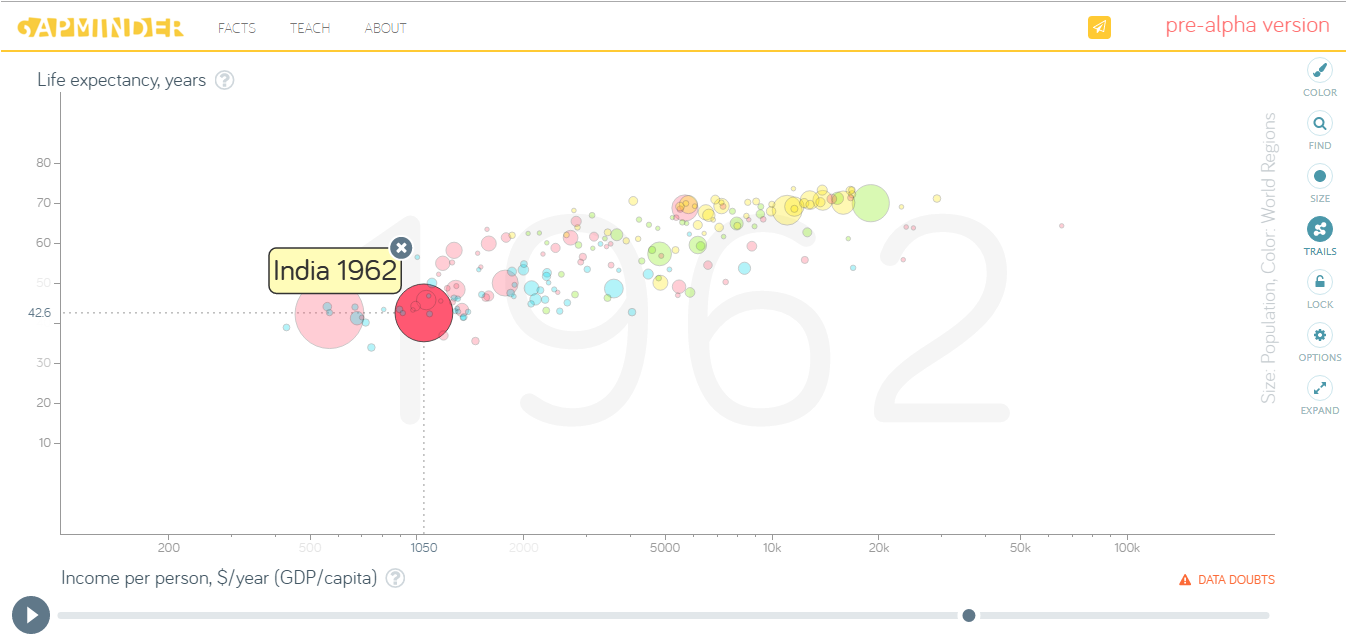
\includegraphics[scale=.4]{image/gapminder}
    \caption{Đồ thị trực quan dữ liệu Gapminder World}
    \label{fig:gapminder}
	\end{center}
\end{figure}

Như ở hình 2, chúng ta có thể thấy với 1 lượng dữ liệu lớn (ở đây là độ tuổi kỳ vọng ở các quốc gia trên thế giới), có thể được thể hiện trực quan bởi đồ thị bong bóng (bubble chart). Qua kích thước các bong bóng, có thể thấy sự tương quan khác biệt giữa các quốc gia như thế nào. Hay khi trỏ vào 1 bong bóng, chúng ta thấy được số liệu chi tiết ở quốc gia đó, như trong hình là độ tuổi kỳ vọng ở Ấn Độ, vào năm 1962 là 42.6. Ngoài ra ở phía dưới đồ thị, có 1 thanh thể hiện dòng thời gian (timeline), khi thanh thời gian trượt đi, kích thước các quả bóng thay đổi theo như số liệu tương ứng ở các năm của các quốc gia.
%----------------------------------%

%----------------------------------%
\myparagraph{Phương pháp}
Gapminder sử dụng D3.js, một thư việc JavaScript phổ biến trong việc thao tác với các thành phần của một trang web (Document Object Model) dựa trên dữ liệu. 

D3 cho phép thể hiện dữ liệu thông qua HTML, SVG và CSS. D3 còn là một tiêu chuẩn web cung cấp hầu hết các khả năng mà một trình duyệt hiện đại mang lại, mà không cần phải tự viết lại hay dựa trên một nền tảng khuôn khổ. Kết hợp các thành phần trực quan mạnh mẽ và hướng tiếp cận dữ liệu để thao tác trên DOM.
%----------------------------------%

%----------------------------------%
\myparagraph{Đánh giá}
Với mục tiêu luôn luôn cập nhật các công cụ cũng như dữ liệu, nhằm đảm bảo tính xác thực, và đúng đắn của ứng dụng, Gapminder World đảm bảo nguồn dữ liệu chính xác nhất và cập nhật nhất.
Dữ liệu đề tài sẽ sử dụng từ Gapminder để đảm bảo nguồn thông tin luôn xác thực và thể hiện đúng đắn nhất các xu hướng phát triển toàn cầu.

Ngoài ra, cách sử dụng các biểu đồ con để hiển thị dữ liệu liên quan của một đối tượng được tương tác giúp người dùng dễ dàng nắm bắt được chính xác các thông tin muốn truyền đạt, tăng tính thân thiện cũng như trải nghiệm người dùng. Áp dụng tính hiệu quả trên, đề tài đề xuất sử dụng cách thể hiện trải nghiệm người dùng (UI/UX) kế thừa các đặc tính của Gapminder World. 

Về thư viện D3.js được sử dụng trong Gapminder World, đây là một thư viện mạnh mẽ tiếp cận dữ liệu dựa trên các thao tác với DOM. D3.js cho phép tái sử dụng các thành phần và trình nhúng (plugin) một cách đơn giản và hiệu quả. Đề tài đề xuất sử dụng D3.js làm thư viện chính để hiện thực thư viện tương tác giữa các đồ thị.
%----------------------------------%
\subsubsection{Global Health Atlas - WHO}
%----------------------------------%
\myparagraph{Giới thiệu}
Trong một môi trường điện tử, WHO’s Communicable Disease Global Atlas được dùng cho việc phân tích và so sánh dữ liệu chuẩn, thống kê các bệnh truyền nhiễm ở các quốc gia, vùng lãnh thổ, và toàn thế giới. Việc phân tích và biểu diễn dữ liệu ngày càng được hỗ trợ tốt hơn thông qua các thông tin về dân số, điều kiện kinh tế xã hội, và các yếu tố môi trường. Với việc làm đó, biểu đồ Atlas này có thể cho biết được những yếu tố gây ra bệnh truyền nhiễm (2007)\cite{gha}.
\begin{figure}[htp]
    \begin{center}
    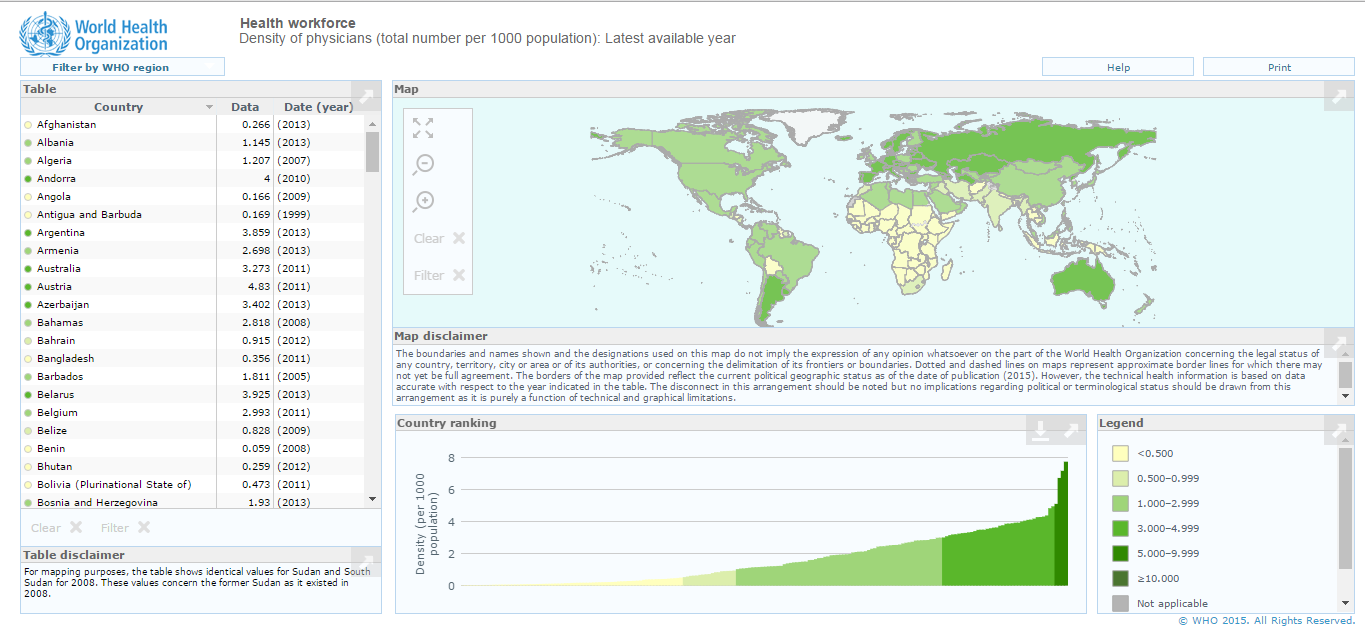
\includegraphics[scale=.4]{image/globalatlas}
    \caption{Biểu đồ tương tác về mật độ bác sĩ của WHO}
    \label{fig:globalatlas}
    \end{center}
\end{figure}
%----------------------------------%

%----------------------------------%
\myparagraph{Mục tiêu}
Ban đầu, với mục đích cung cấp những dữ liệu, báo cáo về các bệnh truyền nhiễm chính (sốt rét, HIV/AIDS,..), thì ngày nay Global Atlas của WHO cũng dùng để phân tích, biểu diễn, so sánh dữ liệu từ những vấn đề liên quan đến y tế khác như: mật độ bác sĩ, số lượng người chết do tai nạn giao thông, tuổi thọ trung bình,… 
%----------------------------------%

%----------------------------------%
\myparagraph{Phương pháp}
Trực quan dữ liệu thành nhiều dạng biểu đồ khác nhau, các biểu đồ có thể tương tác với nhau giúp cho việc nhìn nhận, phân tích, đánh giá thông tin một cách chính xác, đầy đủ.

Ứng dụng\cite{ghaex} bao gồm các thành phần:

\begin{list}{}{}
\item[•] \emph{Bảng dữ liệu:} Được lấy từ database của WHO.
\item[•] \emph{Bản đồ (Map):} Dùng thư viện Google Maps, kết hợp với bảng dữ liệu để tạo ra biểu đồ.
\item[•] \emph{Biểu đồ cột:} Dựa vào bảng dữ liệu để tạo ra biểu đồ.
\item[•] \emph{Chú thích:} Phân vùng dữ liệu.
\end{list}

Tính năng: Ứng dụng hỗ trợ tương tác giữa các biểu đồ, bảng dữ liệu

\begin{list}{}{}
\item[•] Khi click vào một hàng trong bảng dữ liệu (hình 4), bên map sẽ phóng to đến vùng tương ứng, bên biểu đồ cột sẽ nổi bật cột tương ứng. Các tương tác sẽ được thể hiện tương tự khi click vào các biểu đồ.

\begin{figure}[htp]
    \begin{center}
    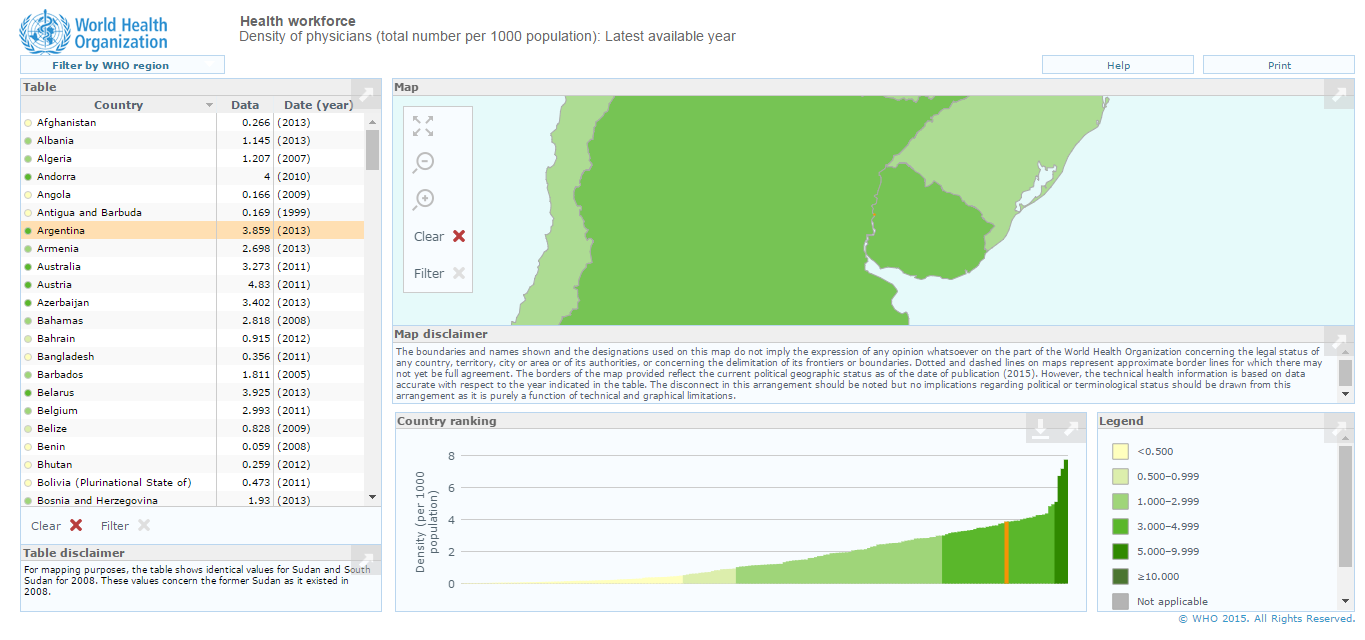
\includegraphics[scale=.4]{image/clickatlas}
    \caption{Tương tác khi click vào một hàng trong bảng dữ liệu}
    \label{fig:clickatlas}
    \end{center}
\end{figure}

\item[•] Khi hover lên một hàng trong bảng dữ liệu (hình 5), bên các biểu đồ cũng sẽ được làm nổi bật vùng tương ứng như khi click, nhưng với 1 màu sắc khác (bên map sẽ không phóng to đến vùng tương ứng).
\end{list}

\begin{figure}[htp]
    \begin{center}
    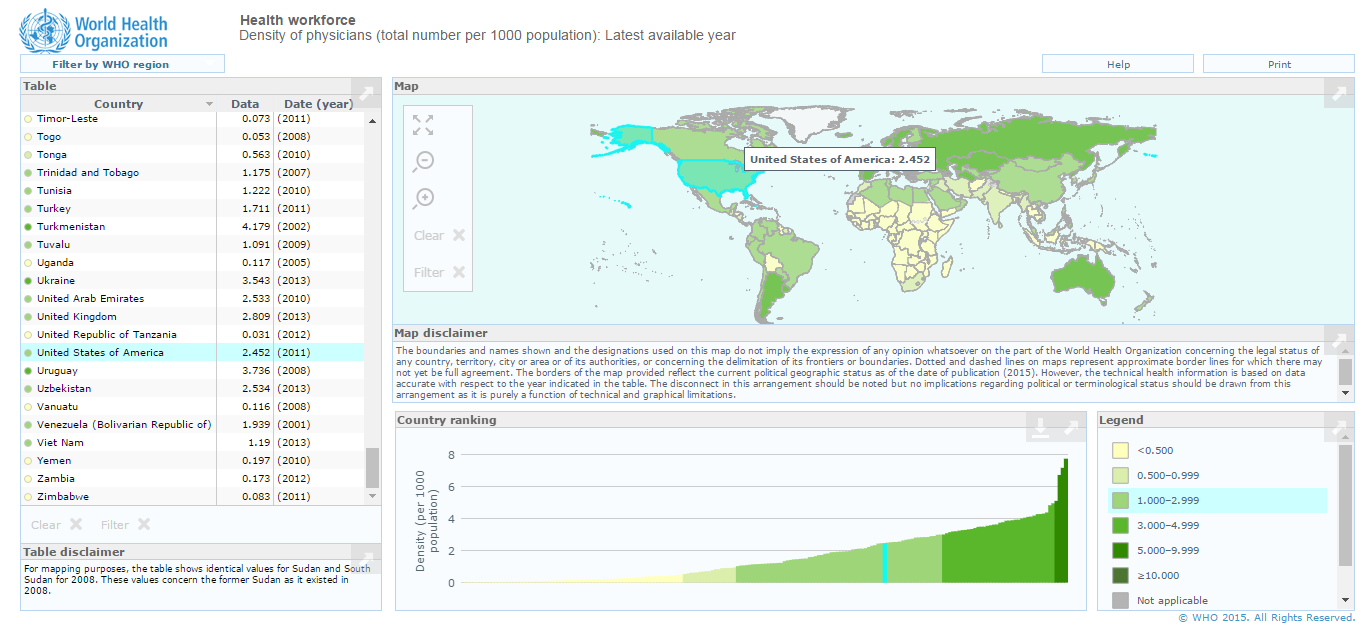
\includegraphics[scale=.4]{image/hoveratlas}
    \caption{Tương tác khi hover lên Map}
    \label{fig:hoveratlas}
    \end{center}
\end{figure}
%----------------------------------%

%----------------------------------%
\myparagraph{Đánh giá}
Dữ liệu được WHO thu thập trên toàn thế giới, cập nhật theo thời gian, đảm bảo tính chính xác của ứng dụng.

Bên cạnh đó, việc trực quan thành nhiều loại biểu đồ, thể hiện được nhiều cái nhìn khác nhau của dữ liệu giúp đánh giá vấn đề 1 cách đúng đắn, đầy đủ.

Một tính năng khác đó là việc tương tác giữa các giữa các đồ thị giúp người dùng có nhiều cái nhìn từ nguồn dữ liệu, hiểu được thông tin rút trích từ các đồ thị, tăng tính thân thiện, trải nghiệm của người dùng.

Do đó, đề tài đề xuất sử dụng nhiều đồ thị để biểu diễn cho nguồn dữ liệu đầu vào, và sự tương tác giữa các đồ thị.
%----------------------------------%
\subsubsection{Thư viện đồ thị C3.js}
%----------------------------------%
\myparagraph{Giới thiệu}
C3.js là một thư viện mã nguồn mở \cite{c3js} dựa trên thư viện D3.js , nhằm cho phép người dùng có cái nhìn sâu hơn về các ứng dụng web tích hợp đồ thị.

Toàn bộ mã nguồn của thư viện nằm ở: \url{https://github.com/masayuki0812/c3}
\begin{figure}[htp]
	\begin{center}
    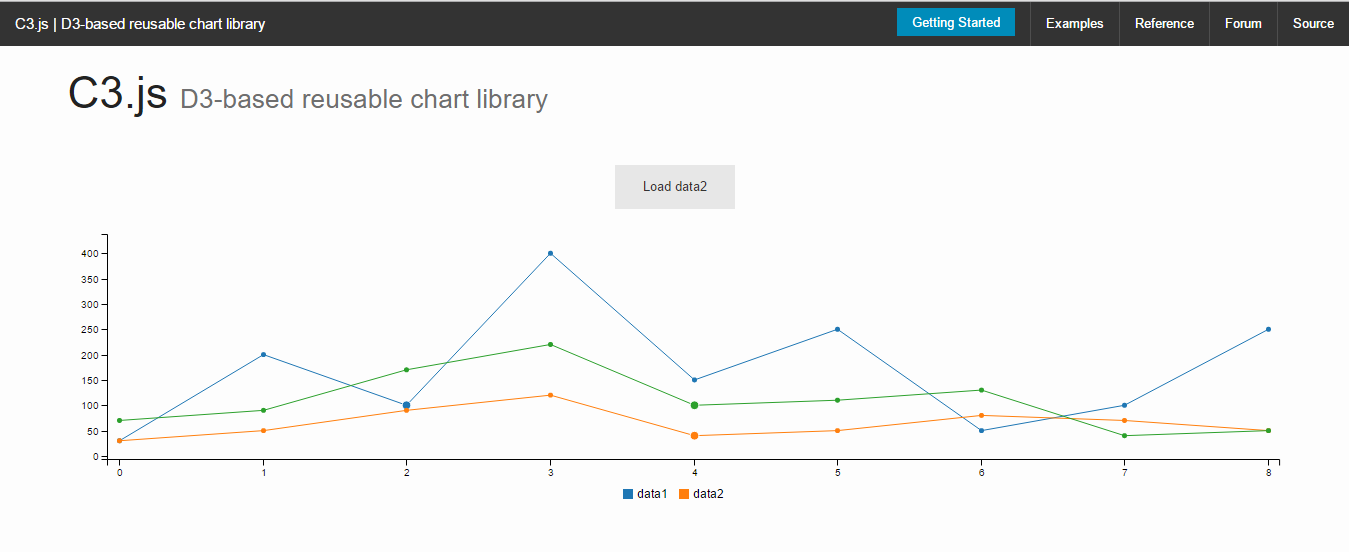
\includegraphics[scale=.4]{image/c3js}
    \caption{Thư viện đồ thị C3js}
    \label{fig:c3js}
	\end{center}
\end{figure}
%----------------------------------%

%----------------------------------%
\myparagraph{Mục tiêu}
\begin{itemize}
    \item[•] \emph{Sự thoải mái (Comfortable):} C3 giúp người dùng có thể dễ dàng tạo một đồ thị dựa trên D3 bằng cách gộp chung các đoạn code cần thiết để cấu trúc một đồ thị hoàn chỉnh. Qua đó, người dùng không cần phải viết các đoạn code D3 rườm rà như trước nữa.
    
\begin{figure}[htp]
	\begin{center}
    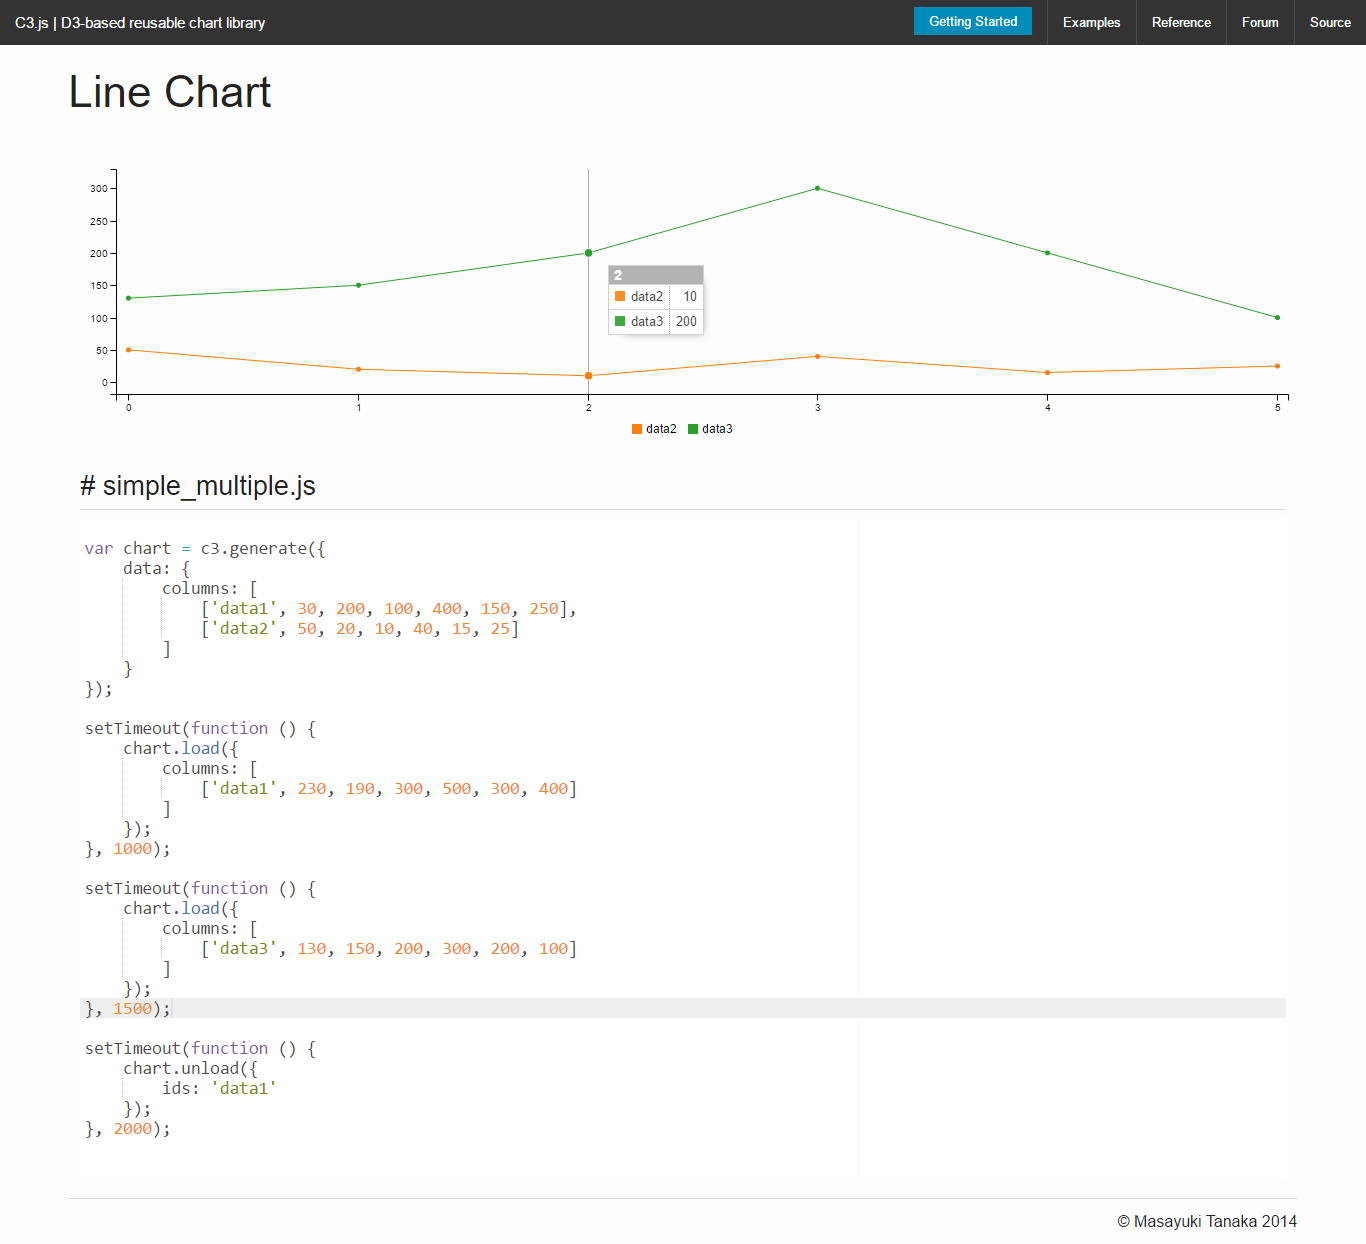
\includegraphics[scale=.3]{image/c3syntax}
    \caption{Thư viện đồ thị C3js}
    \label{fig:c3syntax}
	\end{center}
\end{figure}

[Hình 6] Thông qua một số câu lệnh định nghĩa dữ liệu, C3 khởi tạo một đồ thị cho phép tương tác một cách trực quan thông qua hover, click,.. các thành phần của đồ thị.

    \item[•] \emph{Khả năng tuỳ chỉnh (Customizable):} C3 cung cấp các class tương ứng cho mỗi đối tượng trong đồ thị khi khởi tạo. Qua đó, người dùng có thể định nghĩa các style theo ý muốn theo class cũng như mở rộng cấu trúc các thành phần của đồ thị (trục dữ liệu, hình dạng hiển thị, kiểu đồ thị,.. ) một cách trực tiếp.
    
\begin{figure}[htp]
	\begin{center}
    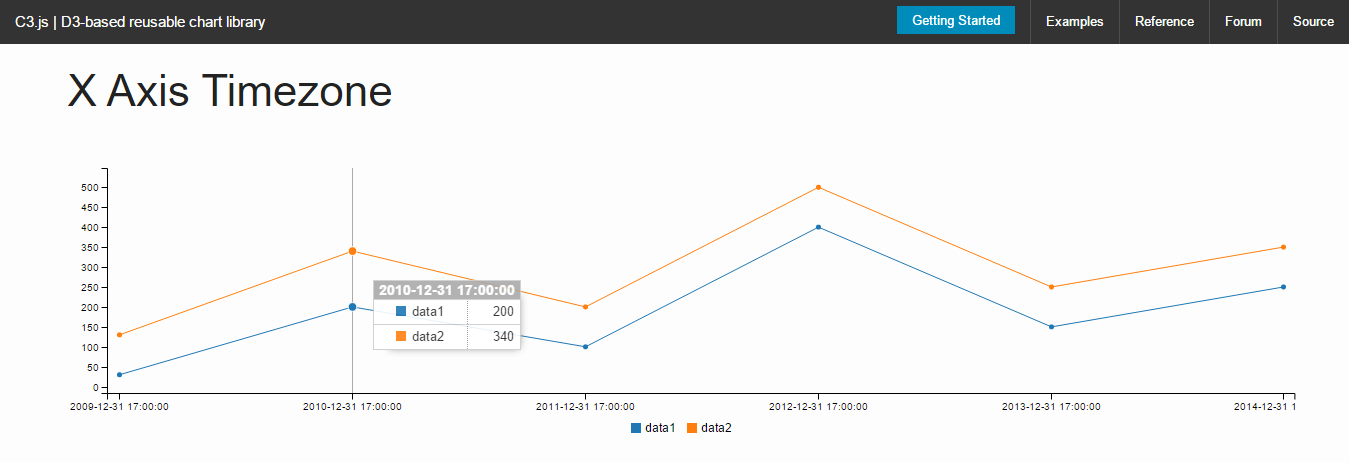
\includegraphics[scale=.4]{image/c3custom}
    \caption{Thư viện đồ thị C3js}
    \label{fig:c3custom}
	\end{center}
\end{figure}    
  
(Hình 7) Trục hoành của đồ thị được tuỳ chỉnh theo thời gian hiện tại với định dạng hoàn toàn tuỳ thuộc người sử dụng.
 
    \item[•] \emph{Khả năng kiểm soát (Controllable):} C3 cung cấp đa dạng các APIs và các hàm callback để truy xuất trạng thái của đồ thị. Bằng cách đó, người dùng có thể cập nhật lại đồ thị thậm chí sau khi đồ thị đã được thể hiện. [Hình 8] Thể hiện một số thành phần được hỗ trợ bởi thư viện C3js.
    
\begin{figure}[htp]
	\begin{center}
    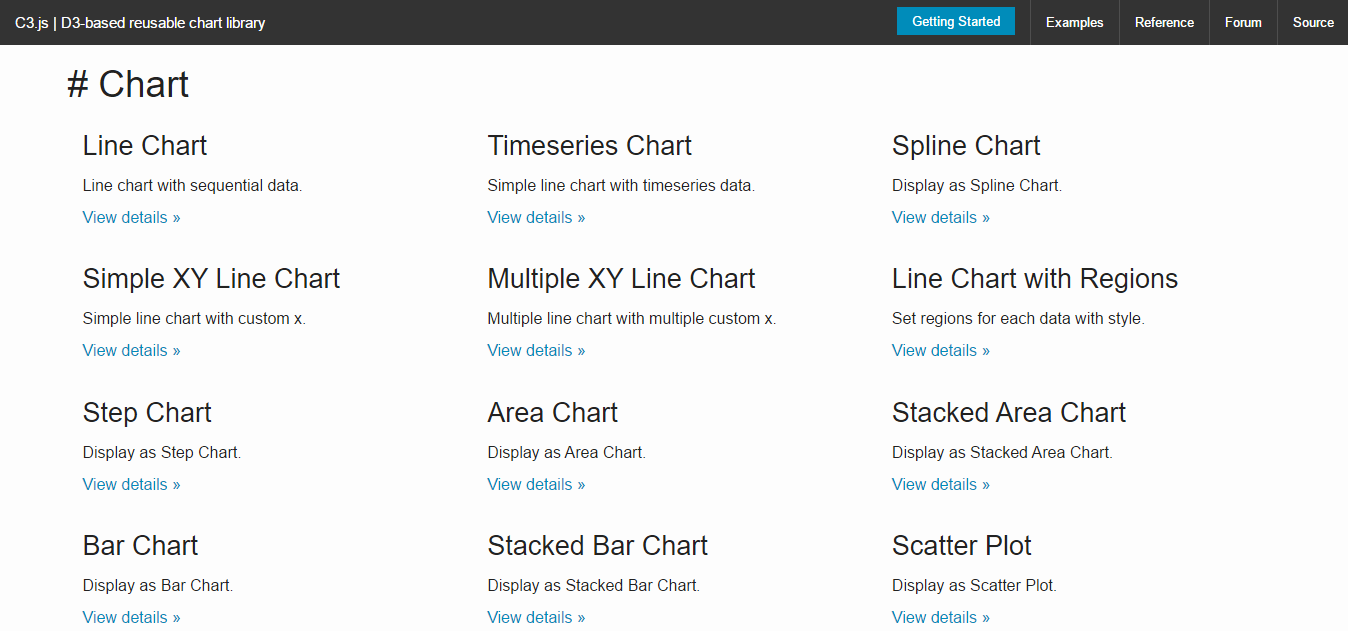
\includegraphics[scale=.4]{image/c3apis}
    \caption{Thư viện đồ thị C3js}
    \label{fig:c3apis}
	\end{center}
\end{figure}

\end{itemize}
%----------------------------------%

%----------------------------------%
\myparagraph{Phương pháp}
Như đã trình bày ở trên, C3js sử dụng thư viện D3js nhằm tạo các đồ thị có khả năng tái sử dụng, cũng như giúp người dùng đào sâu hơn vào khái niệm trực quan dữ liệu thông qua đồ thị trên nền ứng dụng web.

Ngoài ra dựa theo cấu trúc mã nguồn mà C3js chia sẻ, có thể thấy cấu trúc tổ chức của C3js theo hướng hướng đối tượng, được tổ chức theo các class (trục, dữ liệu, đồ thị,.. ) và các phương thức, thuộc tính đi kèm class.

\begin{figure}[htp]
	\begin{center}
    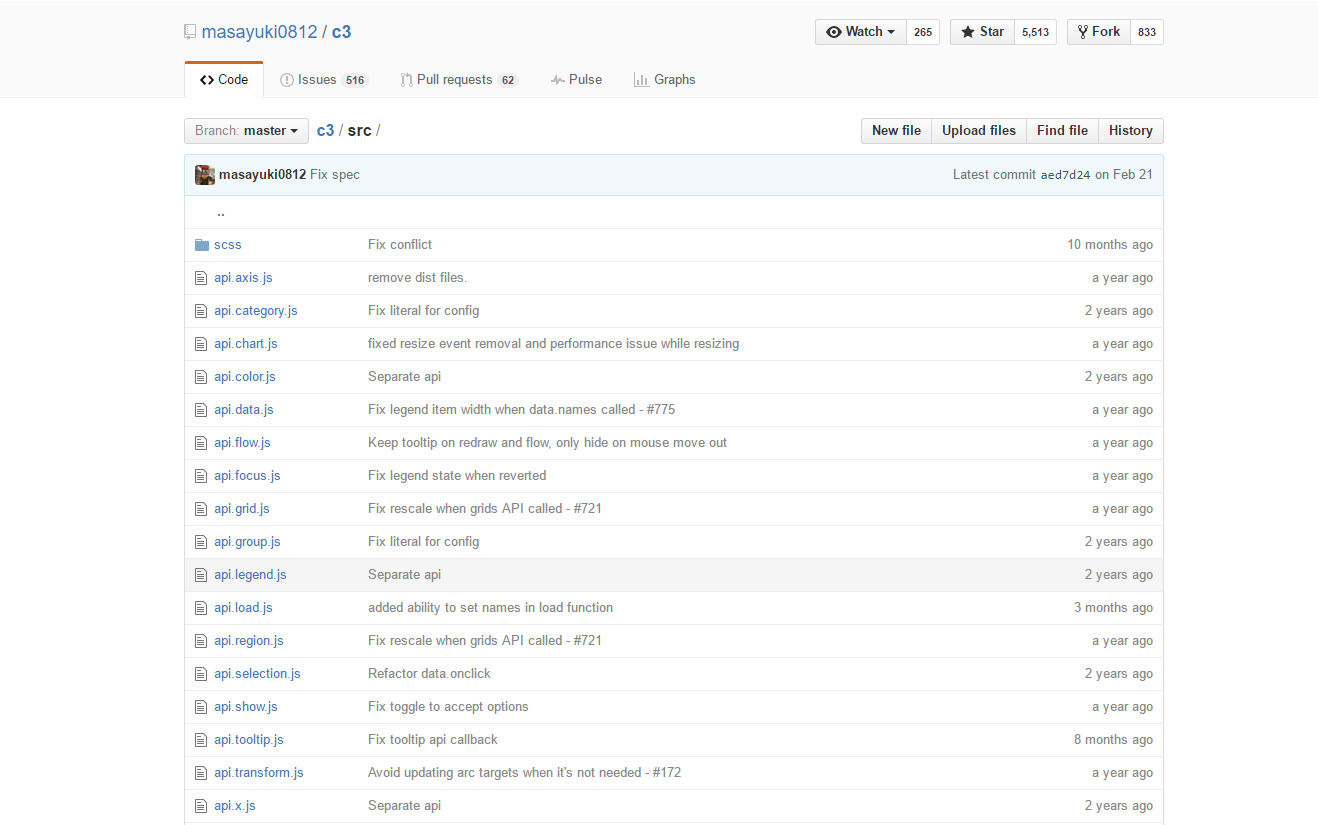
\includegraphics[scale=.4]{image/c3source}
    \caption{Thư viện đồ thị C3js}
    \label{fig:c3source}
	\end{center}
\end{figure}
%----------------------------------%

%----------------------------------%
\myparagraph{Đánh giá}
Cách tổ chức và hiện thực theo hướng hướng đối tượng như trên giúp tiết kiệm số dòng mã, tận dụng khả năng tái sử dụng, đồng thời giúp việc mở rộng về sau rất hiệu quả.

Đề tài đề xuất sử dụng cách hiện thực API theo hướng như thư viện C3js.

%----------------------------------%
\subsubsection{Ứng dụng tạo bản đồ online Mapme}
%----------------------------------%
\myparagraph{Giới thiệu}
Mapme\cite{mapme} là một ứng dụng cho phép người dùng tạo bản đồ, dữ liệu đươc xử lý trực tiếp từ các file Excel đầu vào. Bản đồ tạo ra có các marker tương ứng với dữ liệu, có khả năng tương tác trực tiếp thông qua các sự kiện định nghĩa trước. Ngoài ra, bản đồ được tạo ra còn có thể được nhúng vào các trang web khác thông qua một đoạn mã nhúng. Đặc biệt toàn bộ tương tác từ những bước khởi tạo bản đồ đầu tiên, đến lúc xuất thành quả, đều không yêu cầu người dùng phải viết một dòng mã nào.

\begin{figure}[htp]
	\begin{center}
    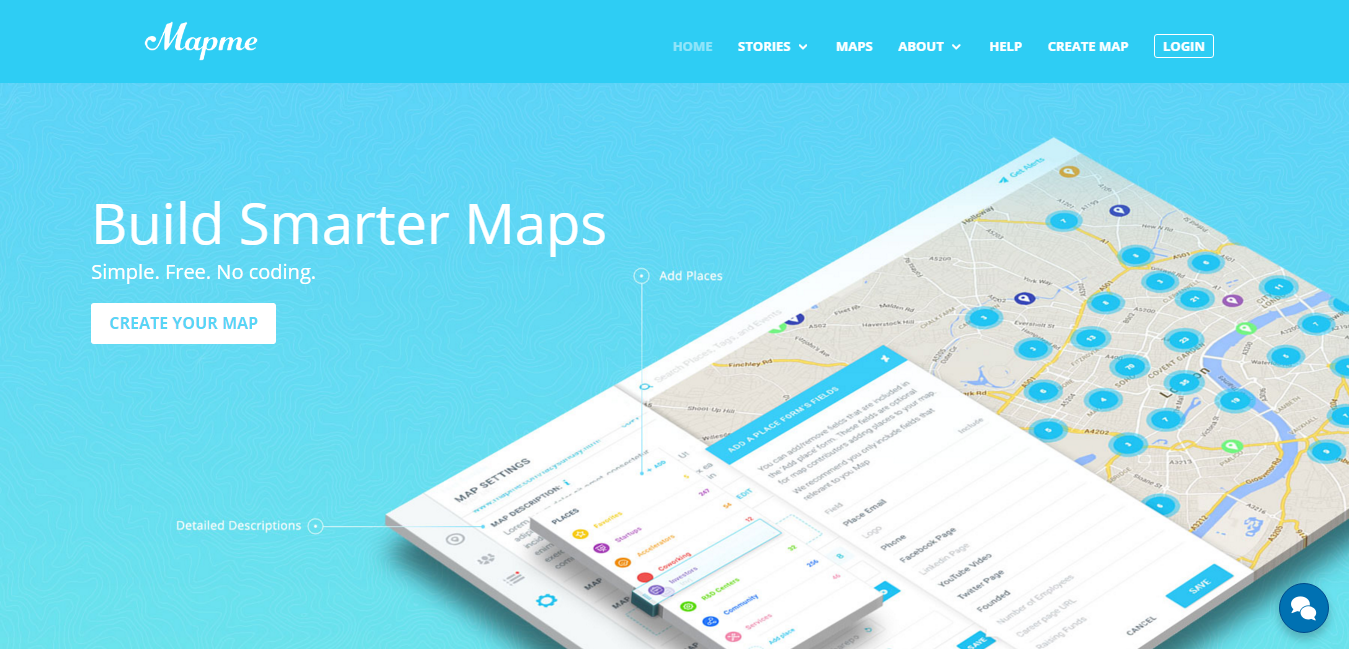
\includegraphics[scale=.4]{image/mapme}
    \caption{Ứng dụng tạo bản đồ online Mapme}
    \label{fig:mapme}
    \end{center}
\end{figure}
%----------------------------------%

%----------------------------------%
\myparagraph{Mục tiêu}
Đầu tiên nói đến các đối tượng mà Mapme hướng tới, đó là các tổ chức, chính phủ, các doanh nghiệp hay các tổ chức cộng đồng phi lợi nhuận.

Phục vụ trong các lĩnh vực khác nhau như giáo dục, các sự kiện, xuất bản hay truyền thụ cảm hứng trong đời sống hằng ngày.
%----------------------------------%

%----------------------------------%
\myparagraph{Phương pháp}
Sử dụng OpenStreetMap (viết tắt OSM)\cite{osm}, một dịch vụ bản đồ thế giới trực tuyến với nội dung mở, nhằm mục đích cung cấp dữ liệu địa lý do nhiều người cùng cộng tác với nhau trên hệ thống Wiki. Nó thường được gọi "Wikipedia của bản đồ". Dự án OSM được sáng lập năm 2004, chủ yếu để cạnh tranh với các công ty và cơ quan chính phủ cung cấp dữ liệu địa lý theo các điều khoản sử dụng được coi là quá chặt chẽ. OSM cho phép ứng dụng cập nhật dữ liệu địa lý trực tuyến một cách chính xác, luôn được cập nhật nhằm đảm bảo các dữ liệu luôn đi sát thực tế nhất.

\begin{figure}[htp]
	\begin{center}
    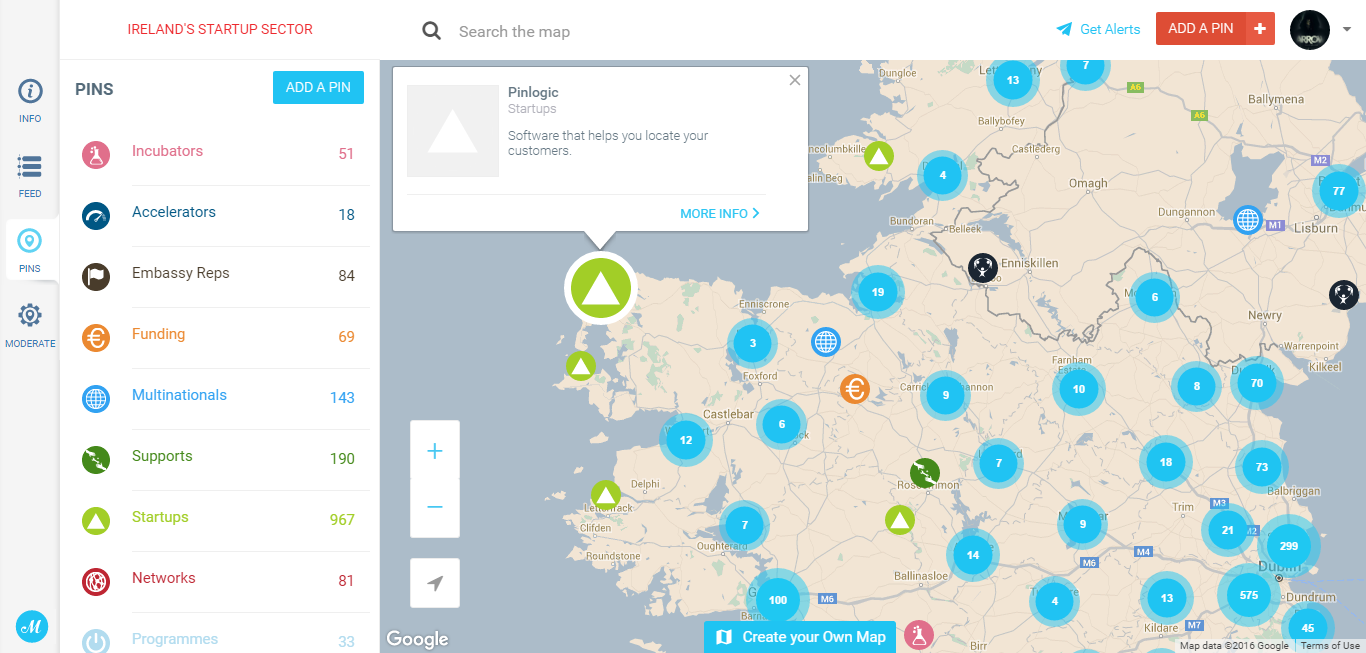
\includegraphics[scale=.4]{image/mapmeOSM}
    \caption{Ứng dụng tạo bản đồ online Mapme}
    \label{fig:mapmeOSM}
	\end{center}
\end{figure}

Như hình 11 có thể thấy, các thông tin về khởi nghiệp ở quốc gia Ireland được trực quan thông qua các biểu tượng (marker). Cùng với đó là các số liệu tương ứng được xử lý trực tiếp từ các file Excel đầu vào.
Ngoài ra, người dùng còn có thể tương tác với các marker này để thể hiện thông tin chi tiết ở các điểm chỉ định.

\begin{figure}[htp]
	\begin{center}
    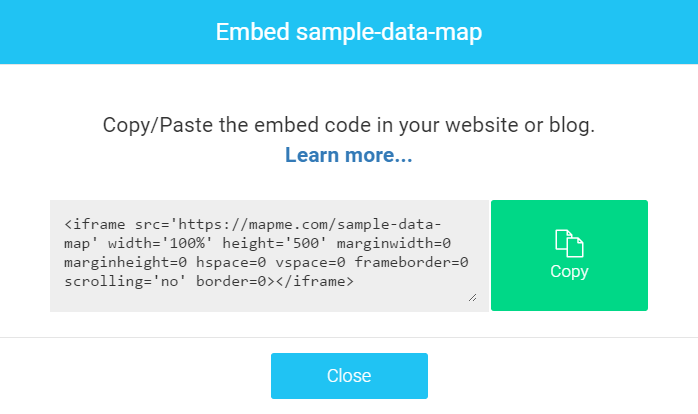
\includegraphics[scale=.8]{image/mapmeExport}
    \caption{Ứng dụng tạo bản đồ online Mapme}
    \label{fig:mapmeExport}
	\end{center}
\end{figure}

Đặc biệt, Mapme còn hỗ trợ sinh mã nhúng [Hình 12], dưới dạng iframe, giúp người dùng nhúng trực tiếp bản đồ mình vừa tạo vào các website tuỳ mục đích.
%----------------------------------%

%----------------------------------%
\myparagraph{Đánh giá}
Đầu tiên là về cách sử dụng OpenStreetMap làm dịch vụ cung cấp bản đồ, đảm bảo ứng dụng luôn chính xác về các dữ liệu địa lý so với thực tế. Nhóm đề tài đề xuất sử dụng OpenStreetMap làm dịch vụ cung cấp bản đồ cho API mà nhóm đề tài thực hiện.

Ngoài ra, ứng dụng cho phép người dùng tương tác trực tiếp với các marker trên bản đồ, hiển thị các thông tin liên quan đến các địa điểm đó. Thay vì phải đọc các dữ liệu thô theo vùng miền, theo quốc gia, vùng lãnh thổ như trước, cách tương tác này giúp người dùng dễ dàng cập nhật thông tin cũng như có cái nhìn tổng quan, khả năng so sánh giữa các địa điểm khác nhau mà không phải chăm chú vào các con số nhàm chám như trước.
%----------------------------------%

\subsection{Kiến thức nền tảng}
\subsubsection{JavaScript}
%----------------------------------%
\myparagraph{Giới thiệu}
\textbf{JavaScript} là một ngôn ngữ nhẹ (lightweight), thông dịch, hướng đối tượng với first-class function, và được biết đến nhất như là một ngôn ngữ kịch bản (scripting language) cho các trang Web, nhưng \textbf{JavaScript} cũng có thể được sử dụng trong các môi trường non-browser như node.js hay Apache CouchDB. Javascript là một prototype-based, ngôn ngữ kịch bản đa mô hình lập trình (multi-paradigm), động (dynamic), hỗ trợ nhiều kiểu như hướng đối tượng, lập trình mệnh lệnh (imperative programming), và lập trình hàm (functional programming).

Chuẩn cho \textbf{JavaScript} là \textbf{ECMAScript}. Phiên bản hiện nay là \textbf{ECMAScript 7} được công bố vào tháng 6/2016. Tuy nhiên, cho đến hiện nay, các trình duyệt chỉ hỗ trợ chuẩn \textbf{ECMAScript 5}, sắp tới đây sẽ hỗ trợ cho \textbf{ECMAScript 6}. Nhóm sử dụng chuẩn \textbf{ECMAScript 6} như là tiêu chuẩn để coding thư viện. Các tính năng mạnh mẽ của \textbf{ECMAScript 6} sẽ được liệt kê ở những phần sau.
%----------------------------------%

%----------------------------------%
\myparagraph{Tính năng}
\textbf{JavaScript} nâng cao sự linh động và khả năng tương tác cho website bằng cách sử dụng các hiệu ứng của nó như thực hiện các phép tính, kiểm tra form, viết các trò chơi, bổ sung các hiệu ứng đặc biệt, tuỳ biến các chọn lựa đồ hoạ, tạo ra các mật khẩu bảo mật và hơn thế nữa.

Cụ thể, \textbf{JavaScript} có thể được dùng để:
\begin{list}{}{}
\item[•] \emph{Tương tác với người dùng:} Chúng ta có thể viết mã để đáp lại các sự kiện. Các sự kiện này sẽ có thể phát sinh bởi người dùng: nhấp chuột hay được phát sinh từ hệ thống, định lại kích thước của trang …
\item[•] \emph{Thay đổi nội dung động:} Mã JavaScript có thể dùng để thay đổi nội dung và vị trí các phần tử một cách động trên một trang nhằm đáp lại sự tương tác với người dùng.
\item[•] \emph{Kiểm tra tính hợp lệ dữ liệu:} Chúng ta có thể viết mã nhằm kiểm tra tính hợp lệ của dữ liệu do người dùng nhập vào trước khi nó được gửi lên Web server để xử lý.
\end{list}
%----------------------------------%

%----------------------------------%
\myparagraph{ECMAScript 6}
ECMAScript 6 hay gọi tắt là ES6 hay ES2015, đây là phiên bản nâng cấp, tập hợp các kỹ năng nâng cao của Javascript. ES6 ra đời năm 2015 nên cái tên ES2015 được lấy làm tên chính thức với nhiều tính năng mới học hỏi các ngôn ngữ cấp cao khác, hy vọng dần theo thời gian Javascript trở thành một ngôn ngữ lập trình hướng đối tượng.

Một số tính năng mạnh mẽ của ES6:
\begin{list}{}{}
\item[•] \emph{Classes:} Với việc hỗ trợ class, các cú pháp trông đẹp đẽ, đơn giản, dễ nhìn, rõ ràng hơn rất nhiều  trong việc tạo ra đối tượng và giải quyết vấn đề thừa kế.
\item[•] \emph{Modules:} Hỗ trợ import/export các giá trị (biến, hàm, …) từ/đến các module.
\item[•] \emph{Block Scoped:} Khai báo biến với từ khóa let để cho biết biến này chỉ tồn tại trong phạm vi block của nó.
\item[•] \emph{Destructuring Assignment:} Dễ dàng khởi tạo các biến trong suốt các câu lệnh gán từ một mảng.
\item[•] \emph{Arrow function}
\item[•] \emph{Default Parameter Values:} Cho phép gán giá trị mặc định cho tham số.
\item[•] \emph{Rest Parameter:} Kết hợp các argument còn lại thành một tham số của hàm.
\end{list}
%----------------------------------%

%----------------------------------%
\myparagraph{Ứng dụng}
Dựa trên những đặc điểm và khả năng mạnh mẽ trong hỗ trợ lập trình API của JavaScript đã kể trên, nhóm đề xuất sử dụng JavaScript làm ngôn ngữ chính để hiện thực API.

Ngoài ra, nhóm đề xuất sử dụng chuẩn ECMAScript 6 làm tiêu chuẩn cho các ràng buộc, quy tắc (coding conventions) khi hiện thực API.
%----------------------------------%
\subsubsection{D3.js}
%----------------------------------%
\myparagraph{Giới thiệu}
D3.js được viết bởi Mike Bostock, là 1 thư viện JavaScript dùng để thao tác với document dựa trên dữ liệu (data). D3 giúp mang dữ liệu đến cuộc sống bằng cách sử dụng HTML, SVG, và CSS. Sức mạnh của D3 trên chuẩn web cung cấp đầy đủ các tính năng của những trình duyệt hiện đại mà không buộc mình vào một khuôn khổ nhất định nào, kết hợp với các thành phần trực quan mạnh mẽ và một phương pháp hướng dữ liệu để thao tác DOM (Document Object Model).

D3 không phải là framework giải quyết mỗi vấn đề riêng biệt nào, thay vào đó D3 giải quyết điểm cốt lõi của vấn đề: sự thao tác hiệu quả các document dựa trên dữ liệu. Do đó, D3 có được sự linh hoạt cao, có thể sử dụng toàn bộ các tính năng của các tiêu chuẩn web như HTML, SVG, và CSS.

D3 cho phép nhúng bất kì kiểu dữ liệu nào vào 1 phần tử DOM, và sau đó có thể áp dụng CSS3, HTML, và/hoặc SVG lên dữ liệu này. Cuối cùng, D3.js có thể giúp tạo ra dữ liệu tương tác thông qua việc sử dụng những sự biến đổi (transformation), chuyển đổi (transition) hướng dữ liệu của D3.js.
%----------------------------------%

%----------------------------------%
\myparagraph{Tính năng}
Một số tính năng mạnh mẽ của D3:
\begin{list}{}{}
\item[•] \emph{Selections:} Tập hợp các node tùy ý gọi là selections, và D3 sử dụng phương pháp declarative để biến đổi selections này. Đặc biệt D3 cũng áp dụng các selectors được định nghĩa bởi W3C Selectors API, nhờ đó các phần tử sẽ được chọn lựa ra một cách dễ dàng.
\item[•] \emph{Dynamic Properties:} Dễ dàng thay đổi các thuộc tính, style một các động thông qua các function trong D3.
\item[•] \emph{Enter và Exit:} Sử dụng enter và exit các selections, người dùng có thể tạo ra nhiều node mới cho các dữ liệu mới và xóa các node mà không cần thiết. Với việc sử dụng đúng những tác vụ cần thiết trên các node sẽ làm tăng hiệu suất và mang đến những hiệu ứng chuyển đổi tuyệt vời hơn.
\item[•] \emph{Transformation:} D3 sử dụng các tiêu chuẩn web: HTML, SVG, và CSS. Do đó nếu trình duyệt giới thiệu một phiên bản mới, người dùng có thể sử dụng D3 ngay lập tức, không yêu cầu cập nhật. Ngoài ra giúp người dùng dễ dàng debug với sự trợ giúp của trình duyệt.
\item[•] \emph{Transitions:} Interpolator của D3 hỗ trợ cả 2 kiểu primitive, ví dụ như là số và số nhúng trong string (font-size, dữ liệu về path, …) và các giá trị phức tạp. Người dùng thậm chí có thể mở rộng interpolator để hỗ trợ cho các thuộc tính phức tạp và cấu trúc dữ liệu.
\end{list}
%----------------------------------%

%----------------------------------%
\myparagraph{Ứng dụng}
D3 được viết bằng JavaScript, và sử dụng kiểu lập trình hàm (functional programming) do đó có thể sử dụng lại code và thêm những hàm chức năng mà người dùng muốn. Điều đó có nghĩa là nó sẽ mạnh mẽ như thế nào là dựa vào người dùng muốn làm ra nó. Cách người dùng chọn để định dạng, thao tác, tương tác với dữ liệu là tùy thuộc ở họ.

D3 rất thích hợp dùng trong đề tài, nó giúp xây dựng framework trực quan dữ liệu mà người dùng muốn, dễ dàng sử dụng, do đó giúp tạo ra API một cách dễ dàng hơn, API dễ hiểu, dễ sử dụng.
%----------------------------------%

\subsubsection{OpenLayers}
%----------------------------------%
\myparagraph{Giới thiệu}
OpenLayers được tạo ra bởi MetaCarta sau hội nghị O'Reilly Where 2.0 (29-30/06/2005) và chính thức phát hành thành mã nguồn mở trước hội nghị  O'Reilly Where 2.0 (13-14/06/2006) bởi MetaCarta Labs. Hai dự án khác về công cụ xây dựng bản đồ phát hành bởi MetaCarta là FeatureServer và TileCache. Từ tháng 11/2007, OpenLayers trở thành dự án mã nguồn mở chính thức của Hội đồng Không gian địa lý.

Sơ qua về OpenLayers, đây là một thư viện JavaScript mã nguồn mở (được chứng nhận bởi BSD License) nhằm phục vụ mục đích biểu diễn thông tin trên bản đồ  đối với các trình duyệt Web, không phụ thuộc phía server. Nó cung cấp API chuyên về xây dựng các ứng dụng địa lý trên nền Web tương tự như Google Maps và Bing Maps, với một điểm khác biệt duy nhất, OpenLayers hoàn toàn miễn phí, được xây dựng và phát triển nên bởi cộng đồng phát triển phần mềm mã nguồn mở. Thư viện xây dựng trên Prototype JavaScript Framework.

Hiện nay, OpenLayers đã ra tới phiên bản OpenLayers 3. OpenLayers 3 được viết lại nhằm dễ hiểu hơn, hướng tới các tính năng của HTML5 và CSS3. Thư viện tiếp tục hỗ trợ trình chiếu, các giao thức tiêu chuẩn và các chức năng chỉnh sửa. Phiên bản mới này tập trung vào cải thiện hiệu năng, xây dựng đơn giản hơn, các thành phần trở nên trực quan hơn, API được cải tiến và còn nhiều hơn nữa.
%----------------------------------%

%----------------------------------%
\myparagraph{Tính năng}
Openlayers có 4 tính năng chính:
\begin{list}{}{}
\item[•] \emph{Thể hiện Lớp dưới dạng ô (Tiled Layers):} Các lớp này được kéo về từ OpenStreetMap (OSM), Bing, MapBox, Stamen, MapQuest và bất cứ nguồn nào mà bạn có thể tìm thấy. Hỗ trợ đa dạng các Layer mà bạn có thể sử dụng trong ứng dụng của mình.
\item[•] \emph{Thể hiện Lớp dưới dạng Vector (Vector Layers):} Sinh ra dữ liệu dạng vector từ GeoJSON, TopoJSON, KML, GML và một số định dạng khác.
\item[•] \emph{Tính đối ứng nhanh gọn (Fast \& Mobile Ready):} Hỗ trợ tùy chỉnh các thành phần một cách nhanh gọn và thuận tiện nhất. Cho phép xây dựng một bản tùy chỉnh gọn nhẹ gồm các thành phần mà lập trình viên cần.
\item[•] \emph{Mài dũa các góc cạnh và dễ dàng tùy chỉnh (Cutting Edge \& Easy to Customize):} Bản đồ sinh ra bởi công nghệ WebGL, Canvas 2D, và từ những tính năng ưu việt nhất của HTML5. Dễ dàng tùy chỉnh style bằng CSS.
\end{list}
%----------------------------------%

%----------------------------------%
\myparagraph{Ứng dụng}
Đề tài hướng tới xây dựng thư viện JavaScript cho phép tương tác giữa bản đồ và các đồ thị dựa trên dữ liệu đầu vào, cho nên OpenLayers, cụ thể OpenLayers 3 sẽ là công cụ đắc lực cho việc xây dựng thành phần bản đồ trong đề tài.
%----------------------------------%

\subsubsection{Webpack}
%----------------------------------%
\myparagraph{Giới thiệu}
Webpack là một mô-đun đóng gói (module bundler) rất mạnh. Một gói (bundle) là một tập tin Javascript mà kết hợp với các tài nguyên đi chung với nhau và nên được gửi trả về client trong một phản hồi cho một tập tin yêu cầu duy nhất. Một bundle có thể bao gồm các dạng tập tin như Javascript, CSS, HTML, và hầu hết bất kì loại tập tin khác.

Có 4 khái niệm quan trọng (core concept) trong Webpack:

\begin{list}{}{}
\item[•] \emph{Entry:} Webpack tạo ra đồ thị của tất cả các phụ thuộc (dependency) trong ứng dụng. Điểm bắt đầu của đồ thị này chính là điểm đầu vào (entry). Điểm đầu vào nói cho webpack biết được nơi bắt đầu và đi theo đồ thị này để biết cần gộp những gì.
\item[•] \emph{Output:} Một khi đã gộp tất cả các tài nguyên lại với nhau, người lập trình cần nói cho webpack biết nơi đóng gói ứng dụng. Output mô tả cho webpack cách xử lý các mã được gộp.
\item[•] \emph{Loaders:} Mọi tài nguyên trong dự án của người lập trình đều là mối quan tâm của webpack (điều này không có nghĩa là mọi tài nguyên đều được gộp lại cùng với nhau). Webpack xem mỗi tập tin (css, html, scss, jgp, …) như là một mô-đun. Tuy nhiên, webpack chỉ biết Javascript. Loaders trong webpack sẽ chuyển đổi những tập tin này thành những mô-đun khi nó được thêm vào trong đồ thị.
\item[•] \emph{Plugins:} Loaders chỉ thực thi chuyển đổi trên mỗi tập tin, do đó plugins được sử dụng rất phổ biến để thực hiện những hành động và chức năng tùy chỉnh trên các mảnh (chunk) hoặc bộ (compilation) của các mô-đun. Hệ thống plugin của webpack cực kỳ mạnh mẽ và dễ dàng tùy chỉnh.
\end{list}
%----------------------------------%

%----------------------------------%
\myparagraph{Hoạt động và Tính năng}
Webpack quét toàn bộ source code của ứng dụng, tìm kiếm câu lệnh import, xây dựng một đồ thị của những dependency, và cho ra 1 hoặc nhiều bundle. Với 1 số các plugin hỗ trợ, Webpack có thể tiền xử lí (preprocess) và thu gọn (minify) các tập tin không phải Javascript khác nhau như CoffeeScript, Typescript, SASS, và LESS,… và có thể chuyển đổi code từ ES6 sang ES5 để chạy được trên trình duyệt.

Một số tính năng đáng chú ý của webpack:

\begin{list}{}{}
\item[•] Hỗ trợ các module format như AMD, CommonJS thông qua các loader (plug-in) như ES6.
\item[•] Hỗ trợ các package manager như bower, npm
\item[•] Các loader cho dạng không phải code như CSS, template, …
\item[•] Có chế độ chạy trên môi trường phát triển.
\end{list}
%----------------------------------%

%----------------------------------%
\myparagraph{Ứng dụng}
Với các tính năng mạnh mẽ của Webpack, C9js sử dụng Webpack để:

\begin{list}{}{}
\item[•] Chuyển đổi code từ ES6 sang ES5 nhờ vào loader Babel.
\item[•] Đóng gói các tập tin Javascript thành một tập tin duy nhất, dùng cho việc triển khai (release).
\item[•] Hỗ trợ chạy trên môi trường phát triển (development environment).
\end{list}

Một ví dụ về việc áp dụng Webpack trong quá trình phát triển thư viện: Hình \ref{fig:webpack_build} Theo dõi sự thay đổi của các tập tin Javascript, CSS trong quá trình coding để tiến hành build lại thư viện.

\begin{figure}[htp]
	\begin{center}
    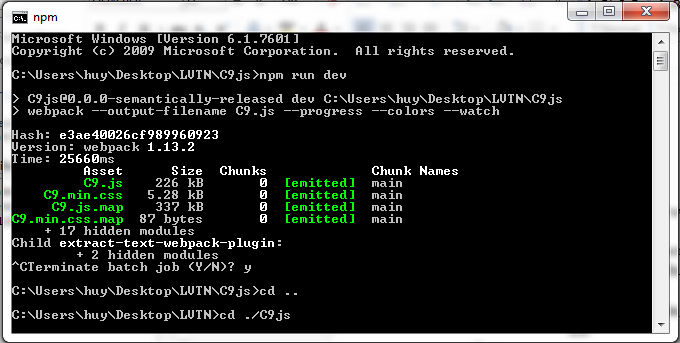
\includegraphics[scale=.8]{image/webpack_build}
    \caption{Theo dõi thay đổi mã nguồn với Webpack}
    \label{fig:webpack_build}
	\end{center}
\end{figure}
%----------------------------------%

\subsubsection{Unit Testing}
Kiểm thử đơn vị (\textbf{Unit Testing}), còn được gọi là kiểm thử thành phần (component testing), tập trung vào việc kiểm tra các phần nhỏ của source code như là class mà người phát triển (developer) viết nên. Những test này có ý nghĩa rất quan trọng trong việc giúp đỡ người phát triển đảm bảo những phần nhỏ trong code chạy đúng theo mong đợi và hoạt động một cách chính xác khi được kết hợp với những phần khác của ứng dụng. Kiểm thử như vậy giúp cho việc quản lí ứng dụng theo thời gian bằng cách đảm bảo những thay đổi do người lập trình tạo ra sẽ không vô tình ảnh hưởng đến những phần khác của hệ thống.

Việc kiểm thử đối với Javascript đang ngày càng trở nên quan trọng đối với người lập trình. Ngày nay, có rất nhiều framework để chọn lựa cho việc kiểm thử. Và C9js đã sử dụng những công cụ sau để thực hiện việc kiểm thử:

\subsubsubsection{Jasmine}
%----------------------------------%
\myparagraph{Các khái niệm liên quan}

\textit{Test-driven development (TDD):}
\begin{list}{}{}
\item[•] Là một phương pháp tiên tiến để phát triển phần mềm bắt đầu với việc phát triển các test cho mỗi một tính năng. Các test có thể chạy không đúng như mong muốn bởi vì nó được phát triển thậm chí trước cả khi phát triển phần mềm. Người lập trình sau đó sẽ phát triển và cấu trúc lại mã để vượt qua được những test này. 
\item[•] Mục tiêu của TDD là khuyến khích các thiết kế đơn giản và tạo ra sự tự tin (Kent Beck), viết mã một cách gọn gàng và chạy được (Ron Jeffries).
\item[•] TDD liên quan đến test-first programming, tức viết test trước khi viết vừa đủ mã để thực hiện test và cấu trúc lại.
\end{list}

\textit{Behavior-driven development (BDD):}
\begin{list}{}{}
\item[•] Là một quá trình phát triển phần mềm được mở rộng từ TDD. BDD kết hợp những kĩ thuật chung và nguyên tắc của TDD để cung cấp cho việc phát triển phần mềm cũng như quản lý các đội (team) với các công cụ được chia sẽ và một quá trình chia sẽ để hợp tác với nhau trong quá trình phát triển phần mềm.

\item[•] Mục tiêu của BDD là tập trung vào việc lấy được hiểu biết rõ ràng về hành vi của phần mềm thông qua thảo luận với các bên liên quan. BDD viết các test bằng ngôn ngữ tự nhiên giúp cho người không phải là lập trình viên cũng có thể đọc được. Các lập trình viên sẽ sử dụng ngôn ngữ thuần túy của họ để mô tả mục đích mã (code) mà họ viết. Điều này sẽ giúp cho các lập trình viên tập trung vào vấn đề tại sao mã này nên được viết ra, chứ không phải về vấn đề kĩ thuật, và giảm thiểu tối đa vấn đề dịch thuật giữa các ngôn ngữ.
\end{list}
%----------------------------------%
%----------------------------------%
\myparagraph{Giới thiệu về Jasmine}
Jasmine là một framework theo mô hình BDD (behavior-driven framework), tức là sự phát triển hướng theo hành vi cho Javascript, dùng cho việc kiểm thử mã Javascript. Jasmine không phụ thuộc vào bất kì framework Javascript nào, không yêu cầu DOM, và cú pháp của Jasmine rất gọn gàng, rõ ràng, dễ dàng viết các test.
%----------------------------------%
%----------------------------------%
\myparagraph{Đặc điểm}
Để thấy được đặc điểm, cũng như các điểm mạnh, điểm yếu của Jasmine, chúng ta sẽ so sánh nó với một framework phổ biến khác dùng cho việc kiểm thử, đó là Mocha.

\begin{list}{}{}
\item[•] \emph{API:} 
API của Jasmine và Mocha tương tự như nhau. Người lập trình viết bộ mô tả kiểm thử (test suite) với những khối (block) describe và với mỗi testcase, hay còn gọi là một đặc tả (spec), thì sử dụng hàm it.

\begin{lstlisting}[caption=Cấu trúc của một test-suite trong Jasmine,label={code:jasmine_1}]
describe('calculator add()', function() {
	it('should add 2 numbers together', function() {
		// assertions go here
	});
});
\end{lstlisting}

Sự khác nhau bắt đầu đến từ các hàm khẳng định hoặc kỳ vọng (assertion or expectation). Mocha không có thư viện khẳng định (assertion library) được xây dựng sẵn (có thể dùng một số thư viện hỗ trợ thêm như: Chai, should.js, expect.js,…), trong khi đó Jasmine thì hầu như có mọi thứ được xây dựng sẵn.

\begin{lstlisting}[caption=Ví dụ sử dụng expect trong Jasmine,label={code:jasmine_2}]
expect(calculator.add(1, 4)).toEqual(5);
\end{lstlisting}

\item[•] \emph{Kiểm tra đôi (test doubles):}
Test doubles thường được so sánh với đôi đóng thế (stunt doubles), tức là khi thay thế một object bằng một object khác dùng cho mục đích kiểm thử, tương tự như cách các diễn viên được thay thế bởi diễn viên đóng thế trong các cảnh hành động nguy hiểm.

Trong Jasmine, test doubles có hình thái của spy. Một spy là một hàm thay thế một hàm cụ thể mà người lập trình muốn điều khiển hành vi của nó trong một test và ghi lại cách mà hàm đó được sử dụng trong suốt quá trình thực thi của test đó.
Ngược lại đối với Mocha, nó không có thư viện cho test double. Thay vào đó người lập trình cần dùng thêm Sinon.

Spy trong Jasmine hầu như làm được mọi thứ cần thiết cho test doubles, do đó người lập trình có thể không cần sử dụng Sinon nếu đang dùng Jasmine, nhưng Jasmine và Sinon có thể được sử dụng chung với nhau nếu người lập trình cần.

\item[•] \emph{Kiểm thử bất đồng bộ:}
Kiểm thử bất đồng bộ trong Jasmine phiên bản 2.x và Mocha là giống nhau.

\begin{lstlisting}[caption=Ví dụ sử dụng Jasmine để kiểm thử bất đồng bộ,label={code:jasmine_3}]
it('should resolve with the User object', function(done) {
	var dfd = new $.Deferred();
	var promise = dfd.promise();
	var stub = sinon.stub(User.prototype, 'fetch').returns(promise);
	
	dfd.resolve({name: 'David'});
	
	User.get().then(function(user) {
		expect(user instanceOf User).toBe(true);
		done();
	});
});
\end{lstlisting}

Ở ví dụ Mã nguồn \ref{code:jasmine_3}, User là một constructor có hàm tĩnh get. Hàm get sử dụng fetch để thực hiện gửi yêu cầu XHR (bất đồng bộ). Ở đây người lập trình muốn kiểm tra khi hàm get thực thi xong, thì giá trị trả về là một instance của User.

\item[•] \emph{Sinon (Sinon Fake Server):}
Một tính năng có trong Sinon nhưng không có trong Jasmine đó là fake server. Điều này cho phép người lập trình có thể thiết lập những phản hồi giả cho những yêu cầu AJAX.

\item[•] \emph{Thực thi các testcase:}
Trong Mocha, người lập trình có thể chạy các test bằng cách viết dòng lệnh như Mã nguồn \ref{code:mocha_test} trong command line:

\begin{lstlisting}[caption=Khởi chạy trình kiểm thử testcase với Mocha,label={code:mocha_test}]
mocha test --recursive --watch
\end{lstlisting}

Trong Jasmine, người lập trình không có tiện ích giống như Mocha. Thay vào đó, người lập trình phải sử dụng những trình chạy test (test runner), và một test runner rất phổ biến đó là Karma, sẽ được trình bày kĩ ở phần tiếp theo.
\\

Tóm lại, Jasmine có hầu hết mọi thứ được xây dựng sẵn bao gồm các thư viện kỳ vọng và các tiện ích test double. Tuy nhiên, Jasmine không có một test runner vì vậy người lập trình cần một công cụ như Karma để làm việc này.
\end{list}
%----------------------------------%

\subsubsubsection{Karma}

%----------------------------------%
\myparagraph{Giới thiệu}
Karma là một môi trường để chạy test (test runner) cho Javascript chạy trên nền Node.js. Karma rất thích hợp để kiểm thử AngularJS hoặc bất kì các dự án Javascript khác. Sử dụng Karma để chạy các test thì người lập trình sẽ dùng một trong những các bộ mô tả kiểm thử Javascript phổ biến như Jasmine, Mocha, Qunit, … và những test đó được thực thi không chỉ trong những trình duyệt khác nhau do người lập trình chọn (Chrome, PhantomJS, Safari,…), mà còn có thể là trên các thiết bị (platform) họ chọn (máy tính để bàn, điện thoại, máy tính bảng). Ở Karma, người lập trình dễ dàng tùy chỉnh, tích hợp với các dịch vụ tích hợp liên tục phổ biến (continuous intergration packages) như Travis CI, Jenkins, Semaphore và có sự hỗ trợ mạnh mẽ về các plugin.

Nhìn chung, Karma có các tính năng tương tự như Webpack: preprocessor, plugin, loader,… Sức mạnh của Karma nằm ở khả năng chạy các test trên các trình duyệt khác nhau. 
%----------------------------------%

%----------------------------------%
\myparagraph{Hoạt động và Tính năng}
Karma sẽ tạo ra một server giả, và sau đó chạy các test ở nhiều loại trình duyệt khác nhau do người dùng chỉ định sử dụng dữ liệu từ server giả đó. Do Karma chỉ là môi trường nên nó cần một framework như Jasmine, Mocha để chạy test. Kết quả của mỗi test trên mỗi trình duyệt sẽ được xem xét và hiển thị thông qua command line để giúp người lập trình có thể nhìn thấy trình duyệt nào và test nào thành công hay thất bại.

Karma có thể làm những việc sau:

\begin{list}{}{}
\item[•] Tạo ra web server.
\item[•] Thực thi lại các test đối với mỗi trình duyệt.
\item[•] Hiển thị kết quả của mỗi test trong console.
\end{list}
%----------------------------------%

\subsubsubsection{PhantomJS}
%----------------------------------%
\myparagraph{Giới thiệu}
PhantomJS là một trình duyệt không có giao diện người dùng nhưng lại cung cấp Javascript API (headless webkit scriptable), làm cho trình duyệt trở nên hữu dụng. Nó có sự hỗ trợ nhanh chóng và thuần túy cho nhiều chuẩn web khác nhau như: xử lí DOM, bộ chọn CSS (CSS selector), JSON, Canvas, và SVG.
%----------------------------------%

%----------------------------------%
\myparagraph{Tính năng}
PhantomJS có các tính năng sau:

\begin{list}{}{}
\item[•] \emph{Chụp ảnh màn hình (screen capture):} Vì PhantomJS sử dụng WebKit, một bố cục thực (real layout) và phần mềm dựng hình (rendering engine), do đó nó có thể chụp hình một trang web. Bởi vì PhantomJS có thể vẽ mọi thứ trên trang web, nên nó có thể được sử dụng để chuyển đổi nội dung không chỉ trong HTML và CSS, mà còn SVG và Canvas.
\item[•] \emph{Kiểm thử (testing):} Đây là một tính năng phổ biến của PhantomJS. Nó phù hợp cho việc kiểm thử dựa trên command line, và là một phần của tích hợp liên tục. PhantomJS được xem như là công cụ phổ biến để chạy các unit test. Những công cụ như Mocha, Casper rất thích hợp khi kết hợp với PhantomJS, vì những công cụ này dựa trên nó.
\item[•] \emph{Giám sát mạng (network monitoring):} Bởi vì PhantomJS cho phép kiểm tra lưu lượng mạng, nên nó phù hợp để xây dựng nên các bản phân tích về hành vi và hiệu suất mạng.
\item[•] \emph{Giả lập trang (page automation):} Do PhantomJS có thể tải và thao tác một trang web, nên nó rất phù hợp để giả lập nên nhiều trang khác nhau.
\item[•] \emph{Giao tiếp giữa các quá trình (inter process communication):} Hỗ trợ việc giao tiếp giữa PhantomJS và các quá trình khác (I/O, HTTP,…).
\end{list}
%----------------------------------%

%----------------------------------%
\myparagraph{Ưu điểm và nhược điểm}
Chúng ta sẽ so sánh với một trình duyệt cũng rất phổ biến trong việc hỗ trợ kiểm thử, đó là jsdom, để tìm ra điểm mạnh cũng như điểm yếu của PhantomJS:

\begin{table}
\begin{tabu} to 1\textwidth { | X[l] | X[l] | X[l] | }
\hline
\textbf{Tiêu chí} & \textbf{PhantomJS} & \textbf{jsdom}\\
\hline\hline
Định nghĩa & Là một trình duyệt hoàn chỉnh (không hỗ trợ giao diện), với kỹ thuật dựng hình (rendering engine) rất cũ và hiếm thấy & Không phải là một trình duyệt hoàn chỉnh, nó không thể bố cục và dựng hình, và cũng không hỗ trợ điều hướng trang. Chỉ hỗ trợ DOM, HTML, canvas, nhiều web API khác (không hỗ trợ SVG), và chạy kịch bản (script)\\
\hline
Môi trường thực thi & Cần một trình thực thi (executable) để chạy PhantomJS, là native-code nên cần được biên dịch thông qua một framework & Hoàn toàn là JavaScript, có thể chạy thông qua NodeJS \\
\hline
Chi phí (overhead) để tải trang & Cao, tốn nhiều thời gian, do đó việc chạy test-case có thể mất vài phút & Mất vài giây với cùng số lượng test-case \\
\hline
Cách thực thi mã nguồn (load script) & Nếu tạo một đoạn mã  để kiểm (test) thử trong PhantomJS, thì test đó sẽ chạy ở một quá trình khác chứ không phải là ở ứng dụng web. Vì vậy khi thực hiện nhiều bước trong test và các bước này phụ thuộc lẫn nhau, khi đó ứng dụng có thể thay đổi DOM trong những bước này & Ngược lại với PhantomJS, các test sẽ nằm trong cùng luồng (thread) với ứng dụng web, do đó nếu test đang thực thi mã Javascript, thì ứng dụng web không thể chạy mã của nó cho tới khi test đó được thực thi xong\\
\hline
\end{tabu}
\caption{So sánh PhantomJS và jsdom}
\label{table:phantomjs_jsdom}
\end{table}
%----------------------------------%

%----------------------------------%
\myparagraph{Ứng dụng}
Hiện nay thì xu hướng sử dụng Mocha/Chai/jsdom ngày càng phổ biến, hiệu suất tốt hơn so với Jasmine/Karma/PhantomJS rất nhiều, đặc biệt là đối với những dự án lớn. Đã có nhiều dự án lớn đi theo mô hình TDD, bắt đầu với Jasmine/Karma/PhantomJS, tuy nhiên sau một thời gian, người ta đã nhận thấy món nợ kĩ thuật (technical debt) trở nên ngày càng lớn do tốc độ chạy của bộ ba này quá chậm khi dự án ngày một lớn hơn, khi đó Mocha/Chai/jsdom là một lựa chọn tốt hơn để giải quyết vấn đề và ngày càng được ưa chuộng.

C9js ban đầu cũng đã sử dụng bộ Mocha/Chai/jsdom để thực hiện việc kiểm thử. Tuy nhiên vì một lí do lớn nhất C9js đã không sử dụng, chính là jsdom không hỗ trợ SVG. Mà đây là thành phần chính trong các biểu đồ, do D3 dựng lên (render). Trong khi PhantomJS có hỗ trợ đầy đủ các chuẩn web, thuận lợi cho việc kiểm thử các thành phần khác nhau.
%----------------------------------%

\subsubsubsection{Istanbul}
%----------------------------------%
\myparagraph{Giới thiệu}
Là công cụ dùng để đo lường mức độ mà mã nguồn (source code) của thư viện, ứng dụng Javascript đã được kiểm thử thông qua các bộ mô tả kiểm thử (test suite), hay còn gọi với một thuật ngữ là code coverage. Istanbul được viết bằng Javascript.

Istanbul sẽ đo đạc số lượng các câu lệnh (statement), nhánh (branch), hàm (function), dòng lệnh (line) đã chạy bằng những test mà người lập trình đã viết nên.

\begin{figure}[htp]
	\begin{center}
    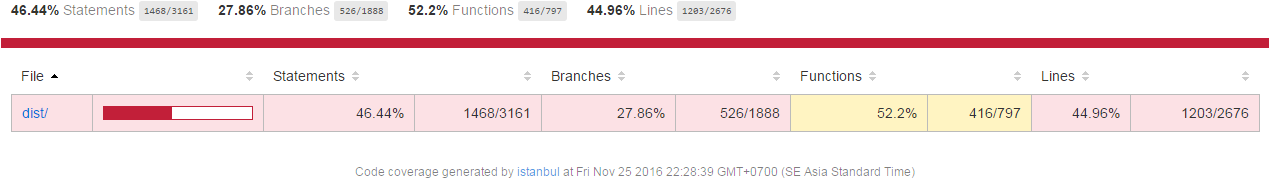
\includegraphics[scale=.5]{image/istanbul_1}
    \caption{Kết quả Unit Testing của C9js được Istanbul tổng quan}
    \label{fig:istanbul_1}
	\end{center}
\end{figure}
%----------------------------------%

%----------------------------------%
\myparagraph{Tính năng}
Các tính năng của Istanbul:

\begin{list}{}{}
\item[•] Theo dõi sự bao phủ (coverage) các câu lệnh, nhánh, và hàm của thư viện Javascript.
\item[•] Module loader sẽ móc nối với các đoạn mã đã được đo đạc trên các kênh (github, codecov,…).
\item[•] Chạy độc lập với trình chạy test (test runner) khi thực hiện kiểm thử đơn vị.
\item[•] Có thể báo cáo kết quả đo đạc qua nhiều định dạng: HTML, LCOV, Cobertuna, …
\item[•] Có khả năng sử dụng những công cụ trung gian (middleware) để kiểm thử tập tin Javascript trên trình duyệt.
\item[•] Có thể được dùng trên command line như là một thư viện (viết dòng lệnh trong command line với istanbul đứng đầu).
\item[•] Kiểm thử rất tốt trên node và trình duyệt.
\end{list}

\begin{figure}[htp]
	\begin{center}
    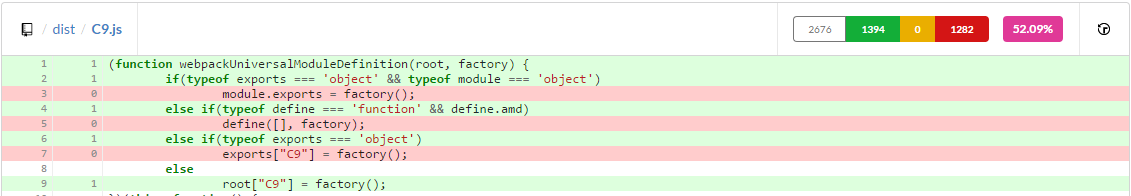
\includegraphics[scale=.5]{image/istanbul_2}
    \caption{Trạng thái các dòng lệnh C9js được cover trên GitHub, báo cáo bởi Istanbul}
    \label{fig:istanbul_2}
	\end{center}
\end{figure}
%----------------------------------%

%----------------------------------%
\myparagraph{Ứng dụng}
Istanbul hỗ trợ bao phủ mã Javascript trong nhiều trường hợp bao gồm kiểm thử đơn vị và kiểm thử chức năng (functional test) ở phía server. C9js áp dụng Istanbul để đo lường mức bao phủ của các câu lệnh, nhánh, hàm trong khi thực hiện kiểm thử đơn vị, đảm bảo tính ổn định và độ tin cậy cho mã nguồn. 

%----------------------------------%

%----------------------------------------------%
%----------------------------------------------%
\newpage
\section{Giới thiệu thư viện C9js}
%----------------------------------%
\subsection{Mô tả bài toán}
Thông qua các công trình đã tìm hiểu, nhóm đề tài đánh giá và trích xuất ra các điểm hạn chế, các vấn đề mà các công trình đó chưa giải quyết được hoặc đã giải quyết nhưng đã lỗi thời cần nâng cấp để phù hợp với bối cảnh hiện tại của các công nghệ Web. Phần đánh giá, so sánh với các công trình liên quan sẽ được thể hiện chi tiết trong mục \textbf{Đánh giá}.

\myparagraph{Bài toán mà nhóm đề tài đặt ra:}
\textit{Hỗ trợ trực quan dữ liệu trên Web thông qua thư viện C9js}.
 
\myparagraph{Các vấn đề \textit{"thắt nút"} cần giải quyết:}
Cũng là các mục tiêu và hướng phát triển \textbf{C9js} đã, đang và mong muốn đạt được: 
\begin{list}{}{}
\item[•] \emph{Hoàn toàn là mã nguồn mở:} \textbf{C9js} là thư viện JavaScript mã nguồn mở, được triển khai thông qua GitHub ở địa chỉ \url{https://github.com/csethanhcong/C9js}.

\item[•] \emph{Kiến trúc xây dựng theo tiêu chuẩn ES2015 (hay ES6):} Nghiên cứu cẩn trọng qua các mã nguồn mở có khả năng trực quan dữ liệu, việc chon kiến trúc để xây dựng từ ban đầu là rất quan trọng, đặc biệt trong khả năng mở rộng nhằm đáp ứng nhu cầu tuỳ chỉnh hay đóng góp từ cộng đồng mã nguồn mở.

\item[•] \emph{Bao gồm các tính năng mới, mạnh mẽ:}
Các tính năng riêng biệt của C9js được thể hiện rõ trên trang chủ của thư viện, tại địa chỉ \url{http://c9js.me/}. Phần trình bày chi tiết sẽ được nêu ở phần sau

\begin{figure}[htp]
	\begin{center}
    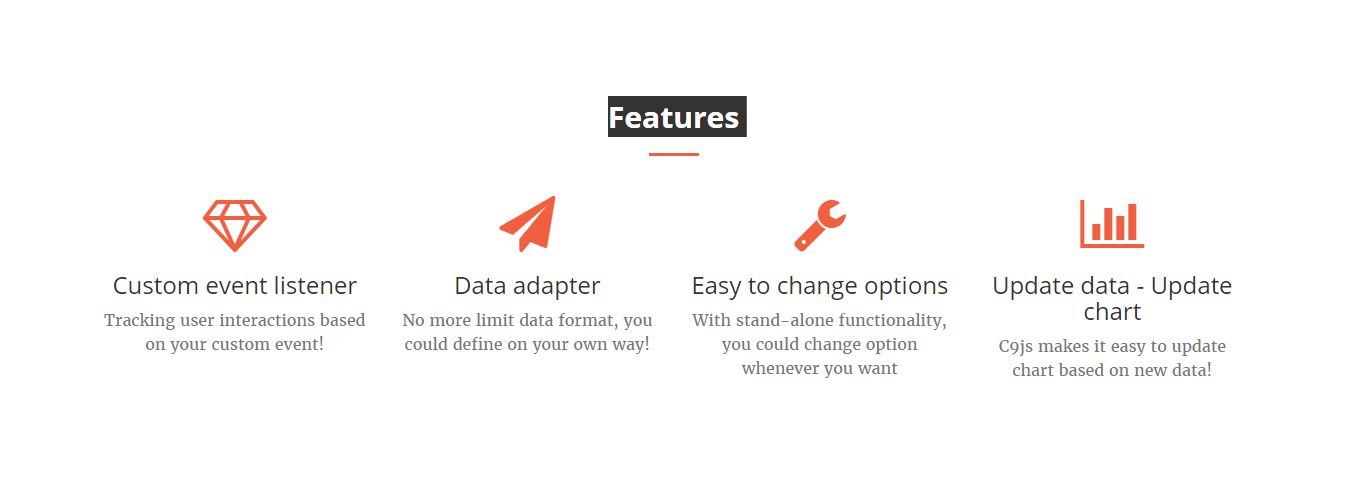
\includegraphics[scale=.5]{image/c9js_feature}
    \caption{Các tính năng chính của C9js trên trang chủ c9js.me}
    \label{fig:c9js_feature}
	\end{center}
\end{figure}

\end{list}

%----------------------------------%
%----------------------------------%
\subsection{Hướng dẫn sử dụng}
Với mong muốn đem lại trải nghiệm nhanh nhất, đơn giản nhất và ít tốn công sức nhất cho người dùng (ở đây là các lập trình viên), nhóm đề tài đã triển khai Website \url{http://c9js.me/} gồm các hướng dẫn từ cơ bản đến chuyên sâu, và gồm cả các ví dụ cụ thể nhất. 

Qua Website c9js.me, có thể thấy mục \textbf{Getting Started} ở các nút ở trang chủ (landing page) hay thông qua menu ở đầu trang như hình \ref{fig:getting_started}

\begin{figure}[htp]
	\begin{center}
    
\includegraphics[scale=.8]{image/getting_started}
    \caption{Menu hướng dẫn trên trang chủ c9js.me}
    \label{fig:getting_started}
	\end{center}
\end{figure}

Khi đó, màn hình hướng dẫn xuất hiện như hình \ref{fig:gs_1}
\begin{figure}[htp]
	\begin{center}
    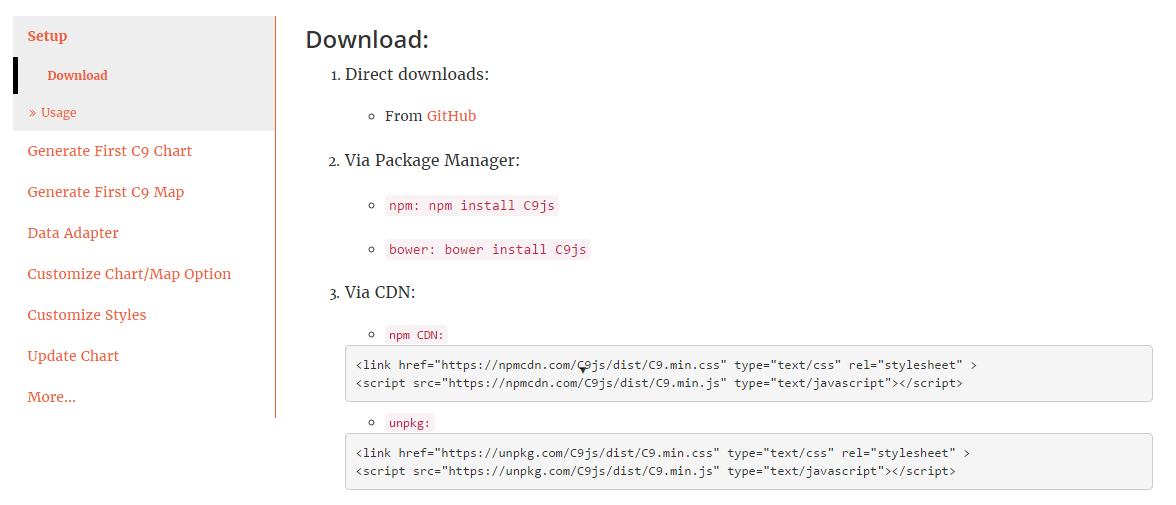
\includegraphics[scale=.5]{image/gs_1}
    \caption{Trang hướng dẫn trên Website c9js.me}
    \label{fig:gs_1}
	\end{center}
\end{figure}

Như có thể thấy, menu giao diện bên trái thể hiện các mục hướng dẫn người dùng, bao gồm các bước cơ bản nhất để sử dụng và tuỳ biến các tính năng trong C9js theo ý muốn

\subsubsection{Cài đặt (Setup)}
\myparagraph{Tải xuống (Download):}
Hiện tại, nhằm đáp ứng tối đa lượng người dùng, C9js được triển khai qua nhiều kênh khác nhau

\begin{list}{}{}
\item[•] \emph{Tải trực tiếp:} Có thể tải trực tiếp ở địa chỉ \url{https://github.com/csethanhcong/C9js/releases/latest}.

\item[•] \emph{Các trình quản lý tập tin (Package Manager):} Hiện tại phổ biến nhất có 2 trình quản lý là \textbf{npm} và \textbf{bower}. Và C9js được phân phối qua cả 2 kênh này. Người dùng cài đặt thông qua một trong các lệnh:

\begin{itemize}
\item[-] \textbf{npm:} npm install C9js
\item[-] \textbf{bower:} bower install C9js
\end{itemize}

\item[•] \emph{Mạng phân phối nội dung (CDN):} Ngoài ra, người dùng còn có thể truy cập các mã nguồn cần thiết từ C9js thông qua hai dịch vụ CDN phổ biến là \textbf{npmcdn} và \textbf{unpkg}

\begin{itemize}
\item[-] \textbf{npmcdn:} 
	\begin{lstlisting}[caption=Tải mã nguồn thông qua \textbf{npmcdn}]
<link href="https://npmcdn.com/C9js/dist/C9.min.css" type="text/css" rel="stylesheet" >
<script src="https://npmcdn.com/C9js/dist/C9.min.js" type="text/javascript"></script>
	\end{lstlisting}

\item[-] \textbf{unpkg:}
	\begin{lstlisting}[caption=Tải mã nguồn thông qua \textbf{unpkg}]
<link href="https://unpkg.com/C9js/dist/C9.min.css" type="text/css" rel="stylesheet" >
<script src="https://unpkg.com/C9js/dist/C9.min.js" type="text/javascript"></script>
	\end{lstlisting}
\end{itemize}

\end{list}

\myparagraph{Cách dùng (Usage):}
Thư viện C9js hỗ trợ tạo biểu đồ dựa trên \textit{d3.js} và bản đồ dựa trên \textit{OpenLayers 3} nên người dùng cần tải các thư viện này trước. 

Tuỳ theo mục đích sử dụng, nếu chỉ dùng chức năng tạo biểu đồ thì chỉ cần tải thư viện \textit{d3.js}, tương tự đối với chức năng tạo bản đồ.

\begin{lstlisting}[caption=Tải mã nguồn \textit{d3.js} trước tiên]
<link href="/path/to/C9.css" rel="stylesheet" type="text/css">
<!-- Load d3.js and C9.js -->
<script src="/path/to/d3.v3.min.js" charset="utf-8"></script>
<script src="/path/to/C9.min.js"></script>
\end{lstlisting}

\begin{lstlisting}[caption=Tải mã nguồn \textit{OpenLayers 3} nếu muốn sử dụng chức năng Bản đồ]
<link rel="stylesheet" href="https://openlayers.org/en/v3.19.1/css/ol.css" type="text/css">
<script src="https://openlayers.org/en/v3.19.1/build/ol.js" type="text/javascript"></script>
<script src="/path/to/C9.min.js"></script>
\end{lstlisting}

\subsubsection{Tạo biểu đồ và bản đồ với C9js}
Sau khi đã tải đầy đủ các tập tin như bước trên, người dùng có thể tạo biểu đồ, bản đồ tương tác với các mã nguồn dựng sẵn.

\myparagraph{Tạo bản đồ cột (Bar Chart):}
C9js đươc nhóm xây dựng dựa trên các tính năng mới nhất của \textit{ES6}, ngoài ra còn mong muốn đem lại sự tiện dụng và rõ ràng cho người dùng.

Đầu tiên, cần tạo một \textit{khung chứa (container)} trong cấu trúc cây \textbf{DOM} của Website.

\begin{lstlisting}[caption=Tạo \textit{container} để chứa biểu đồ]
<div id="chart"></div>
\end{lstlisting}

Sau đó, khởi tạo biểu đồ như Mã nguồn \ref{code:construct_C9js}

\begin{lstlisting}[caption=Khởi tạo biểu đồ với C9js,label={code:construct_C9js}]
var option = {
    id: "chart",
    data: {
        plain: [
            {name: "A", value:  10},
            {name: "B", value:  20},
            {name: "C", value:  50},
            {name: "D", value:  30},
            {name: "E", value:  70},
        ],
    }, 
};
var barChart = new C9.BarChart(option);
barChart.draw();
\end{lstlisting}

Khi đó, trên Website sẽ xuất hiện biểu đồ cột như hình \ref{fig:gs_2}, người dùng có thể tương tác với các thành phần trên đồ thị như \textit{Cột, Chú thích (Legend)} sẽ hiển thị các \textit{Tooltip} chứa các dữ liệu liên quan đến thành phần đang được tương tác..

\begin{figure}[htp]
	\begin{center}
    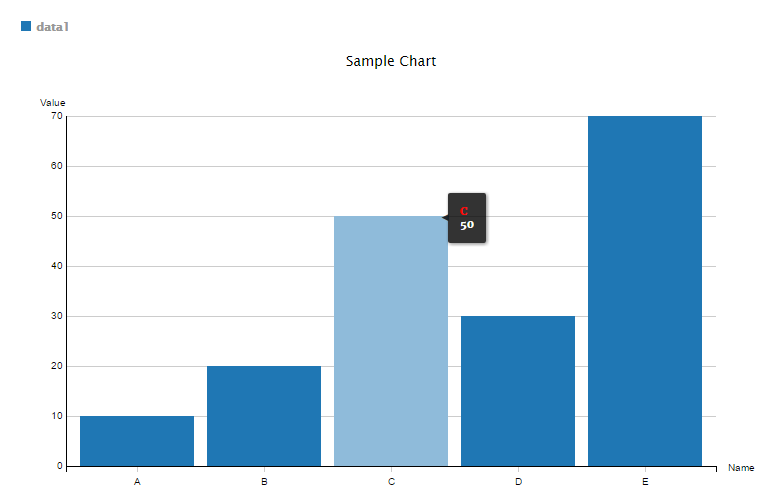
\includegraphics[scale=.7]{image/gs_2}
    \caption{Đồ thị cột từ C9js}
    \label{fig:gs_2}
	\end{center}
\end{figure}

Ngoài ra, C9js còn hỗ trợ tạo nhiều loại đồ thị khác nhau như: \textit{Đồ thị đường (Line Chart), đồ thị thời gian (Timeline), đồ thị tròn (Pie Chart), đồ thị hình xuyến (Donut Chart)}.

\myparagraph{Tạo bản đồ (Map):}
Giống như tạo biểu đồ, đầu tiên người dùng cần tạo một \textit{container} cho bản đồ.

\begin{lstlisting}[caption=Tạo \textit{container} để chứa bản đồ]
<div id="chart"></div>
\end{lstlisting}

Khởi tạo bản đồ tại \textit{container} đó.

\begin{lstlisting}[caption=Khởi tạo bản đồ với C9js]
var option = {
    id: "map",
};
var map = new C9.Map(option);
map.draw();
\end{lstlisting}

Kết quả ta có bản đồ với \textbf{Layer} mặc định là \textit{Tile} cùng \textbf{dữ liệu địa lý} được cung cấp bởi \textit{OpenStreetMap} như hình \ref{fig:gs_3}. Bên cạnh đó, C9js hỗ trợ nhiều loại \textbf{Layer} khác nhau như: \textit{Tile, Vector, Image, VectorTile,...} với nhiều nhà cung cấp \textbf{dữ liệu địa lý} khác nhau như: \textit{OpenStreetMap\citep{osm}, Bing Map\citep{bingmap}, Stamen\citep{stamen}, ...}.

\begin{figure}[htp]
	\begin{center}
    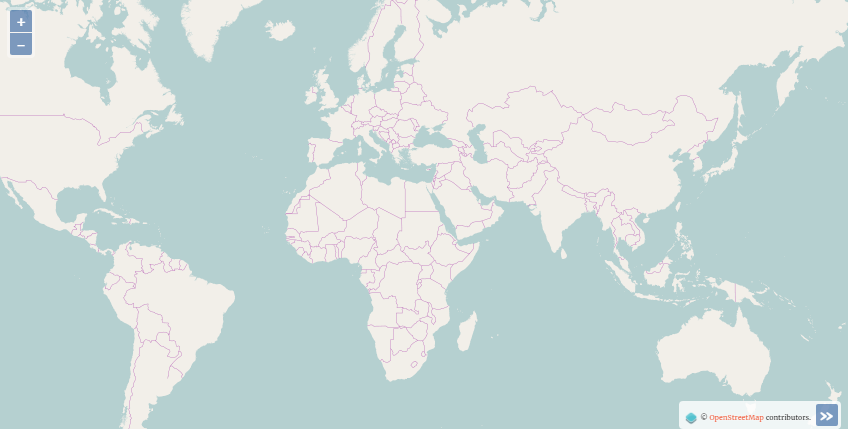
\includegraphics[scale=.7]{image/gs_3}
    \caption{Bản đồ từ C9js}
    \label{fig:gs_3}
	\end{center}
\end{figure}

Hình \ref{fig:gs_3} là bản đồ dạng tĩnh. C9js cho phép người dùng thêm dữ liệu tuỳ biến và tương tác trên bản đồ.

\begin{lstlisting}[caption=Thêm dữ liệu vào Bản đồ với C9js, label={code:gs_map_data}]
var options = {  
    id:"map",
    layers: {
        type: "Image",
        source: {
            name: "ImageVector",
            source: {
                name: 'Vector',
                url: 'https://openlayers.org/en/v3.19.1/examples/data/geojson/countries.geojson',
                format: 'GeoJSON'   
            }
        }
    },
};
var map = new C9.Map(option);
map.draw();
\end{lstlisting}

Như Mã nguồn \ref{code:gs_map_data}, với dữ liệu được truyền vào thông qua địa chỉ bên ngoài (ở đây là dữ liệu các quốc gia được lấy từ \textit{OpenLayers}) bởi thông số \textit{url}. Ta được kết quả như hình \ref{fig:gs_4}. , các giá trị được thể hiện khi đưa chuột (\textit{hover}) lên các vùng trên bản đồ, ở đây là tên các quốc gia trên thế giới.

\begin{figure}[htp]
	\begin{center}
    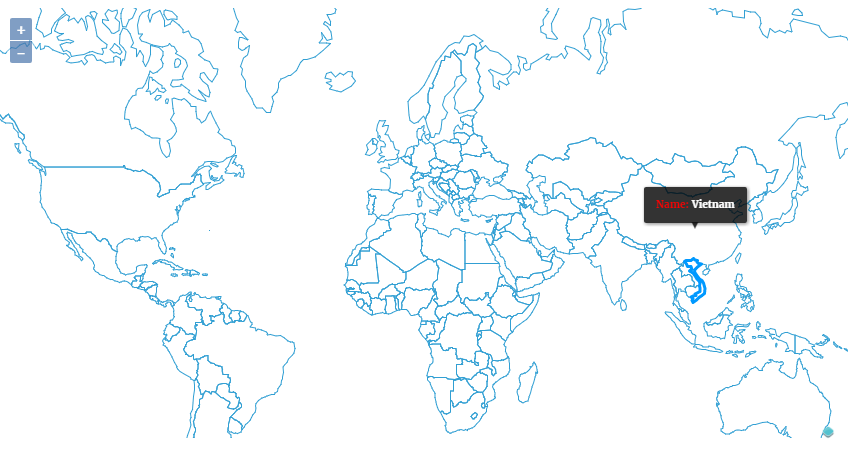
\includegraphics[scale=.7]{image/gs_4}
    \caption{Thêm dữ liệu vào bản đồ với C9js}
    \label{fig:gs_4}
	\end{center}
\end{figure}
%----------------------------------%
%----------------------------------%
\subsubsection{Tuỳ biến định dạng dữ liệu đầu vào}
Với tên gọi là DataAdapter, đây là một trong những tính năng độc đáo và mới lạ của C9js, nhằm tạo điều kiện tốt nhất cho người dùng trong quá trình tiền xử lý dữ liệu đầu vào. Nội dung cụ thể, tính năng và mô hình xây dựng nên DataAdapter sẽ được trình bày chi tiết trong mục \textbf{Kiến trúc xây dựng}.

Quay lại với cách sử dụng tính năng DataAdapter. Trên trang chủ C9js, nhóm có trình bày về khái niệm cở bản để người dùng dễ dàng nắm bắt, cũng như ví dụ sử dụng. DataAdapter hỗ trợ nhiều định dạng dữ liệu khác nhau như \textit{csv (Comma-separated values), tsv (Tab-separated values), json, text, xml} và cả \textit{XHR (XMLHttpRequest)}\cite{xhr}\cite{csv}\cite{tsv}. Thêm nữa, DataAdapter còn cung cấp tính năng tự định nghĩa định dạng dữ liệu đầu vào. Ví dụ ta có một dữ liệu mẫu như Mã nguồn \ref{code:da_1}.

\begin{lstlisting}[caption=Một dữ liệu mẫu với các thuộc tính lồng nhiều cấp, label={code:da_1}]
[
	{
		username: 'Adam',
		property: {
			salary: 1000,
			age: 28,
		},
		...
	},
	...
]
\end{lstlisting}

Khi đó, người dùng chỉ việc định nghĩa các khoá tương ứng \textit{name, value} tuỳ ý, theo bất kỳ trường nào trong dữ liệu mẫu, như ví dụ trên có thể định nghĩa theo các khoá lồng nhiều cấp bằng dấu \textit{"."} (Mã nguồn \ref{code:da_2}).

\begin{lstlisting}[caption=Định nghĩa định dạng dữ liệu đầu vào với C9js, label={code:da_2}]
var option = {
    data: {
        // Your own defined-keys go here
        keys: {
            'name': 'username',
            'value': 'property.salary'
        }
    }
}
var chart = new C9.BarChart(option);
chart.draw();
\end{lstlisting}

\subsubsection{Tuỳ biến kiểu đồ thị}
Việc trực quan dữ liệu có mang tính hiệu quả, hay gây ấn tượng với thị hiếu người dùng hay không hoàn toàn phụ thuộc vào \textit{style} của loại trực quan đó. C9js cho phép lập trình viên toàn quyền tuỳ chỉnh \textit{style} theo ý muốn và mục đích của mình.

Có 3 cách để thay đổi \textit{style} trong C9js:

\begin{list}{}{}
\item[•] \emph{Thông qua các thiết lập (option) tại thời điểm khởi tạo đối tượng Chart/Map}

Mã nguồn \ref{code:option_1} thực hiện các thay đổi về các trục toạ độ (axis), cụ thể là xoay các tick trên trục x 45\degree  (theo chiều kim đồng hồ), không hiện lưới (grid), đối với trục y thực hiện thay đổi nội dung hiển thị trên các tick dựa vào dữ liệu trả về. Ta được kết quả như hình \ref{fig:option_2}.
 
\begin{lstlisting}[caption=Thay đổi \textit{style} tại thời điểm khởi tạo Chart, label={code:option_1}]
var option = {
    axis: {
        x: {
            show: true,
            grid: false,
            tick: {
                rotate: 45
            }
        },
        y: {
            show: true,
            tick: {
                format: function(data, index) {
                    return '-' + data + '-';
                }
            }
        },
    }
};
var chart = new C9.LineChart(option);
chart.draw();
\end{lstlisting}

\begin{figure}[htp]
	\begin{center}
    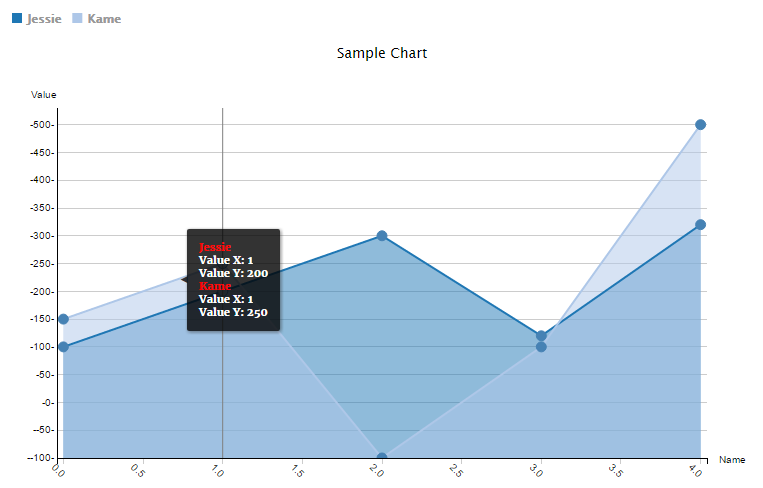
\includegraphics[scale=.8]{image/option_2}
    \caption{Một ví dụ về thay đổi \textit{style} với C9js}
    \label{fig:option_2}
	\end{center}
\end{figure}

\item[•] \emph{Thông qua các CSS Selector được định nghĩa sẵn}

Mỗi thành phần (axis, tick, grid, bar, legend, line, ...) trong C9js đều có các CSS Class\citep{css_class} tương ứng. Lập trình viên có thể thay đổi \textit{style} thông qua các CSS Selector này (Mã nguồn \ref{code:css_class}). Một điểm nhỏ thú vị của C9js nữa là các thành phần liên quan đến màu săc (color, background-color, font-color, ...), giá trị đầu vào có thể dưới dạng tên tiếng Anh, mã RGB hay mã Hex.

\begin{lstlisting}[caption=Thay đổi \textit{style} bằng CSS Selector, label={code:css_class}]
.c9-chart-bar.c9-custom-rect {
    opacity: 0.5;
    background-color: black; // rgb(), hex-code available
}
\end{lstlisting}

\item[•] \emph{Thông qua hàm \textit{setOption}}

Nhằm giảm thời gian và rắc rối khi phải đưa toàn bộ các tuỳ chỉnh, thuộc tính vào lúc khởi tạo, C9js có một tính năng gọi là hàm-đứng-riêng (stand-alone function) \textit{setOption} giúp lập trình viên có thể thay đổi tuỳ chỉnh bất cứ lúc nào sau khi khởi tạo đối tượng Chart/Map. Việc thay đổi được ví dụ như Mã nguồn \ref{code:setoption}, có thể thay đổi các tuỳ chỉnh lồng nhiều cấp bằng phân cách dấu \textit{"."}, tương tự như tính năng DataAdapter đã trình bày ở trên.

\begin{lstlisting}[caption=Thay đổi \textit{style} với \textit{setOption}, label={code:setoption}]
chart.setOption('grid.x.show', true);
\end{lstlisting}

\end{list}

\subsubsection{Cập nhật đồ thị theo dữ liệu}
Một tính năng không thể thiếu đối với trực quan dữ liệu trên nền Web, đó là cập nhật theo thời gian thực. C9js cung cấp API với hàm \textit{updateData} giúp lập trình viên hiện thực điều đó. Ví dụ \ref{code:updatedata_1} thể hiện cách sử dụng \textit{updateData}, ở đây biểu đồ \textit{DonutChart} sẽ được cập nhật lại sau 5 giây với dữ liệu mới được đưa vào, cùng định dạng với dữ liệu ban đầu.

\begin{lstlisting}[caption=Cập nhật lại biểu đồ với \textit{updateData}, label={code:updatedata_1}]
// ... chart drawn already
var chart = new C9.DonutChart(option);
chart.draw();
// Then, update it
setTimeout(function(){
    chart.updateData([
        {name: "Male", value:   45},
        {name: "Female", value: 55},
    ]);
}, 5000);
\end{lstlisting}

Ngoài ra, lập trình viên còn có thể tái định nghĩa lại các khoá-thuộc tính trong lúc cập nhật biểu đồ. Ví dụ ta có mẫu dữ liệu ban đầu được thể hiện dưới dạng biểu đồ tròn (PieChart) với khoá là \textit{age}, sau đó có thể cập nhật lại biểu đồ với cùng mẫu dữ liệu đó, nhưng thể hiện theo khoá \textit{salary} như ví dụ \ref{code:updatedata_2}. Việc này có ý nghĩa giảm tối đa thao tác trên dữ liệu nếu lập trình viên muốn sử dụng lại dữ liệu cũ nhưng chỉ khác khoá mà không cần phải xử lý lại dữ liệu như ban đầu.

\begin{lstlisting}[caption=Định nghĩa lại khoá-thuộc tính trong lúc cập nhật, label={code:updatedata_2}]
setTimeout(function(){
    chart.updateData([
        {
            name: "Male", 
            property: {
                age: 28,
                salary: 5000
            }
        },
        {
            name: "Female", 
            property: {
                age: 30,
                salary: 4500
            }
        },
    ], {
        value: 'property.salary'
    });
}, 5000);
\end{lstlisting}

\subsection{Các ví dụ minh hoạ}
Bên cạnh các hướng dẫn từ cơ bản đến chuyên sâu như trên, nhóm đề tài còn tạo một mục gồm các mã nguồn có sẵn ứng với các tính năng, tuỳ chỉnh và đặc điểm của C9js. Tham khảo tại mục \textbf{Examples} trên trang chủ C9js (Hình \ref{fig:getting_started}). 

Các ví dụ được phân loại theo (Hình \ref{fig:example_page}):

\begin{list}{}{}
\item[•] \emph{Kiểu đồ thị, bản đồ:} BarChart, LineChart, Timeline, DonutChart, PieChart, Map.
\item[•] \emph{Các tiện ích mở rộng:} Axis, Legend, Tooltip, Table.
\item[•] \emph{Các tính năng:} EventListener, DataAdapter, UpdateData.
\item[•] \emph{Các ví dụ mở rộng:} Advance Examples.
\end{list}

\begin{figure}[htp]
	\begin{center}
    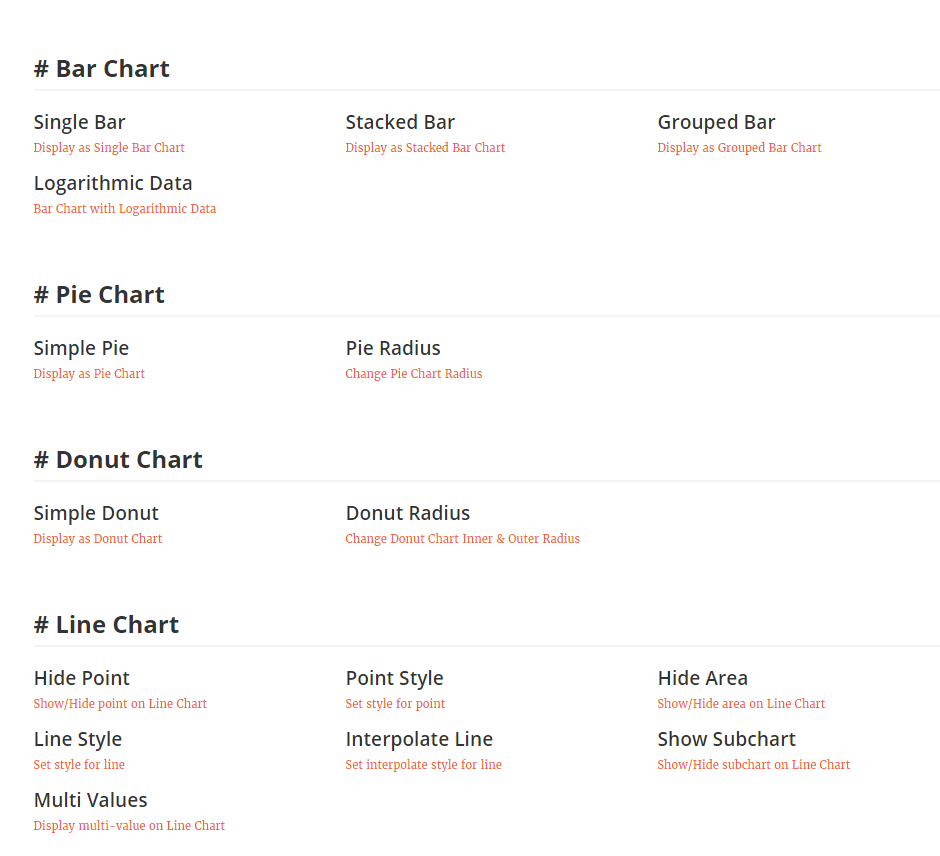
\includegraphics[scale=.6]{image/example_page}
    \caption{Các ví dụ được phân loại theo kiểu đồ thị}
    \label{fig:example_page}
	\end{center}
\end{figure}

Cấu trúc của một trang ví dụ bao gồm ba thành phần (Hình \ref{fig:example_page_2}):

\begin{list}{}{}
\item[1 - ] Biểu đồ, bản đồ được tạo ra.
\item[2 - ] Mã nguồn mẫu.
\item[3 - ] Đường dẫn tới trang \href{https://jsfiddle.net/}{\textit{jsfiddle}} - đây là một trang chỉnh sửa code trực tuyến, nhóm đã để sẵn code mẫu như trên ví dụ và người dùng có thể trực tiếp chỉnh sửa ở \textit{jsfiddle}.
\end{list}

\begin{figure}[htp]
	\begin{center}
    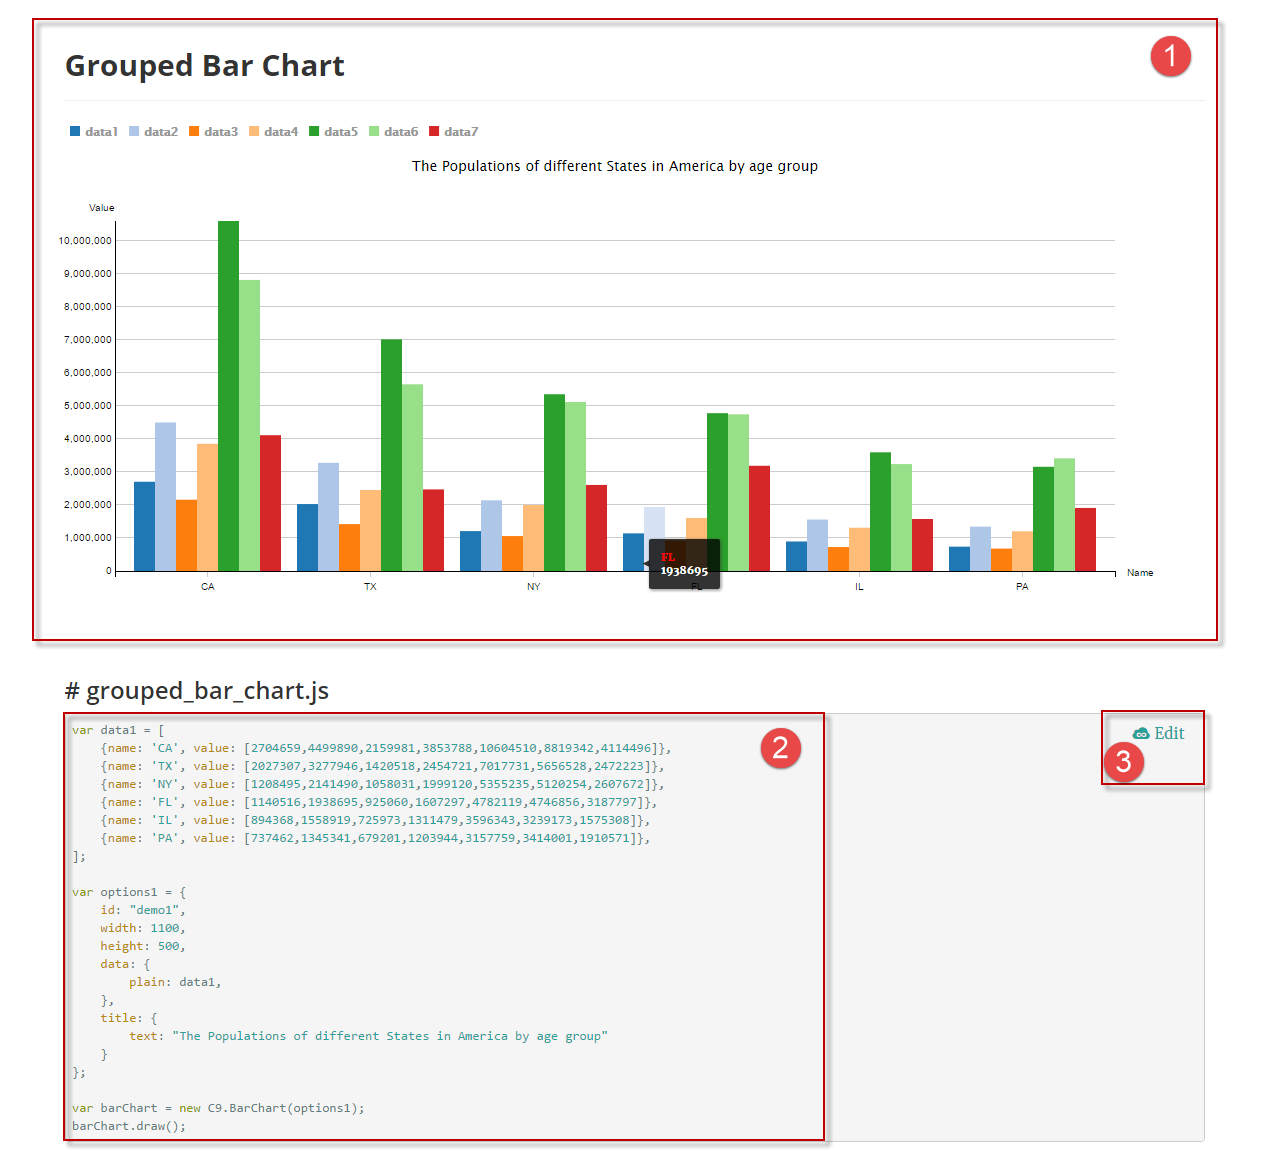
\includegraphics[scale=.5]{image/example_page_2}
    \caption{Cấu trúc một trang ví dụ trên trang chủ C9js}
    \label{fig:example_page_2}
	\end{center}
\end{figure}

Bên cạnh đó, nhóm còn tạo sẵn ví dụ mở rộng: Tương tác giữa bản đồ - biểu đồ (nằm trong mục Advance Examples), một phần nhằm tái hiện ứng dụng Global Health Atlas - WHO\cite{einstein} đã trình bày ở mục \ref{sec:related_work}, một phần muốn giúp người dùng có cái nhìn sâu sắc hơn về tính tương tác trong C9js. Qua đó, có thể tạo các ví dụ mở rộng khác dựa trên mã nguồn mẫu. Như có thể thấy ở hình \ref{fig:advance_1}, có ba thành phần chính được tạo ra: \textit{BarChart, Map, Table}. Khi tương tác với một điểm trên \textit{Map}, \textit{BarChart} sẽ được cập nhật lại dựa trên dữ liệu trả về từ sự kiện tương tác với \textit{Map} - đây là tính năng EventListener của C9js, các tương tác (click, hover, mousemove) trên các thành phần của C9js (Chart, Map) sẽ được trả về dữ liệu tương ứng với điểm đó. Đối với thành phần \textit{Table}, khi hover lên \textit{BarChart}, hàng chứa giá trị tương đương sẽ được làm nổi bật giúp người dùng có cái nhìn trực quan và sinh động đối với dữ liệu.

\begin{figure}[htp]
	\begin{center}
    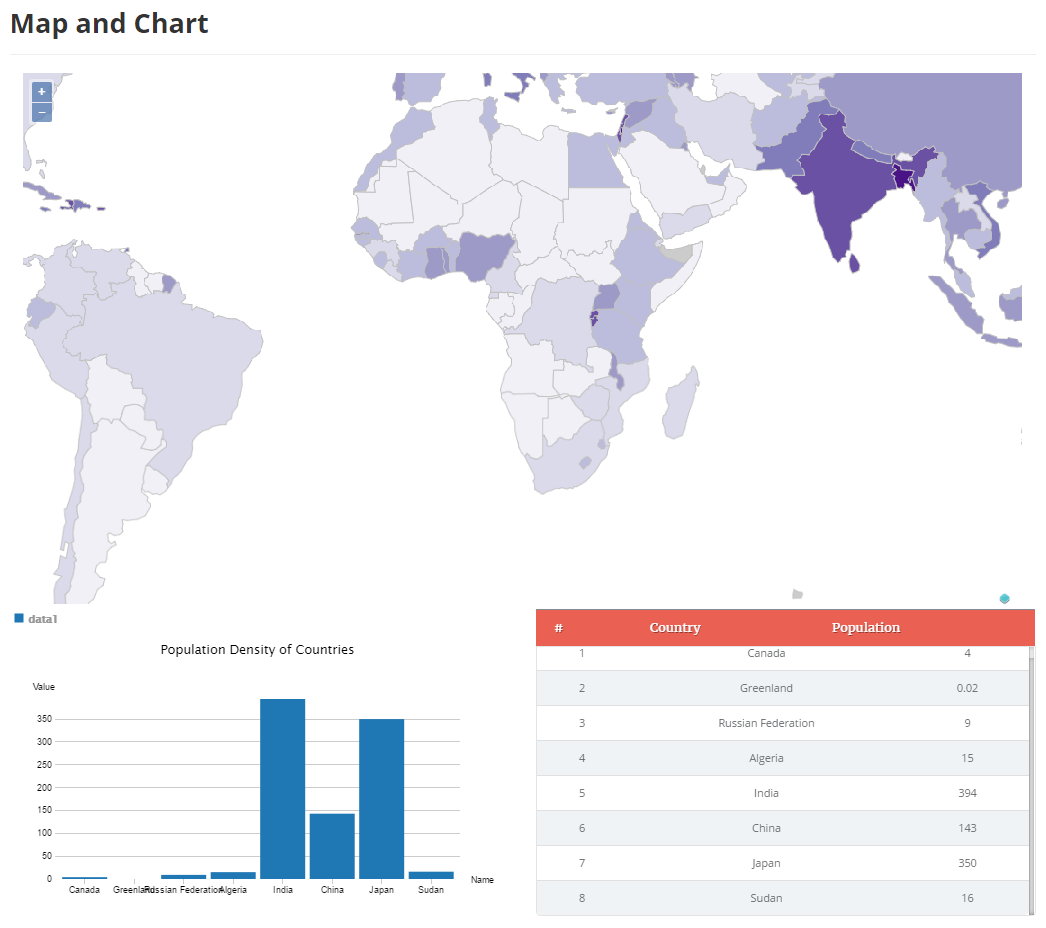
\includegraphics[scale=.6]{image/advance_1}
    \caption{Ví dụ mở rộng tái hiện ứng dụng GHA-WHO}
    \label{fig:advance_1}
	\end{center}
\end{figure}
%----------------------------------%
%----------------------------------------------%
%----------------------------------------------%
\newpage
\section{Quá trình thực hiện}
\subsection{Kiến trúc xây dựng}
\subsection{Hiện thực thư viện}
%----------------------------------------------%
%----------------------------------------------%
\newpage
\section{Kết luận}
\subsection{Đánh giá}
\subsection{Hướng phát triển}
\subsection{Kết luận}
%----------------------------------------------%
%----------------------------------------------%
\newpage
\bibliography{refs}
\bibliographystyle{unsrt}

%----------------------------------------------%

\end{document}
